%%%%%%%%%%%%%%%%%%%%%%%%%%%%%
% Standard header for working papers
%
% WPHeader.tex
%
%%%%%%%%%%%%%%%%%%%%%%%%%%%%%

\documentclass[11pt]{article}



%%%%%%%%%%%%%%%%%%%%%%%%%%
%% TEMPLATES
%%%%%%%%%%%%%%%%%%%%%%%%%%


% Simple Tabular

%\begin{tabular}{ |c|c|c| } 
% \hline
% cell1 & cell2 & cell3 \\ 
% cell4 & cell5 & cell6 \\ 
% cell7 & cell8 & cell9 \\ 
% \hline
%\end{tabular}





%%%%%%%%%%%%%%%%%%%%%%%%%%
%% Packages
%%%%%%%%%%%%%%%%%%%%%%%%%%



% encoding 
\usepackage[utf8]{inputenc}
\usepackage[T1]{fontenc}


% general packages without options
\usepackage{amsmath,amssymb,amsthm,bbm}

% graphics
\usepackage{graphicx,transparent,eso-pic}

% text formatting
\usepackage[document]{ragged2e}
\usepackage{pagecolor,color}
%\usepackage{ulem}
\usepackage{soul}


% conditions
\usepackage{ifthen}


\usepackage{natbib}


%%%%%%%%%%%%%%%%%%%%%%%%%%
%% Maths environment
%%%%%%%%%%%%%%%%%%%%%%%%%%

%\newtheorem{theorem}{Theorem}[section]
%\newtheorem{lemma}[theorem]{Lemma}
%\newtheorem{proposition}[theorem]{Proposition}
%\newtheorem{corollary}[theorem]{Corollary}

%\newenvironment{proof}[1][Proof]{\begin{trivlist}
%\item[\hskip \labelsep {\bfseries #1}]}{\end{trivlist}}
%\newenvironment{definition}[1][Definition]{\begin{trivlist}
%\item[\hskip \labelsep {\bfseries #1}]}{\end{trivlist}}
%\newenvironment{example}[1][Example]{\begin{trivlist}
%\item[\hskip \labelsep {\bfseries #1}]}{\end{trivlist}}
%\newenvironment{remark}[1][Remark]{\begin{trivlist}
%\item[\hskip \labelsep {\bfseries #1}]}{\end{trivlist}}

%\newcommand{\qed}{\nobreak \ifvmode \relax \else
%      \ifdim\lastskip<1.5em \hskip-\lastskip
%      \hskip1.5em plus0em minus0.5em \fi \nobreak
%      \vrule height0.75em width0.5em depth0.25em\fi}



%% Commands

\newcommand{\noun}[1]{\textsc{#1}}


%% Math

% Operators
\DeclareMathOperator{\Cov}{Cov}
\DeclareMathOperator{\Var}{Var}
\DeclareMathOperator{\E}{\mathbb{E}}
\DeclareMathOperator{\Proba}{\mathbb{P}}

\newcommand{\Covb}[2]{\ensuremath{\Cov\!\left[#1,#2\right]}}
\newcommand{\Eb}[1]{\ensuremath{\E\!\left[#1\right]}}
\newcommand{\Pb}[1]{\ensuremath{\Proba\!\left[#1\right]}}
\newcommand{\Varb}[1]{\ensuremath{\Var\!\left[#1\right]}}

% norm
\newcommand{\norm}[1]{\left\lVert #1 \right\rVert}



% argmin
\DeclareMathOperator*{\argmin}{\arg\!\min}


% amsthm environments
\newtheorem{definition}{Definition}
\newtheorem{proposition}{Proposition}
\newtheorem{assumption}{Assumption}

%% graphics

% renew graphics command for relative path providment only ?
%\renewcommand{\includegraphics[]{}}


\usepackage{url}





% geometry
\usepackage[margin=2cm]{geometry}



% changes

\usepackage{soul}
\soulregister\cite7
\soulregister\citep7
\soulregister\ref7

\usepackage[final]{changes}
%\usepackage{changes}


\setaddedmarkup{\textcolor{black}{\hl{#1}}}
\setdeletedmarkup{\textcolor{red}{\sout{#1}}}



\usepackage{CJKutf8}
%\begin{CJK*}{UTF8}{zhsong}
%文章内容。
%\clearpage\end{CJK*}
\newcommand{\cn}[1]{
  \begin{CJK*}{UTF8}{gbsn}
  #1
  \end{CJK*}
}



% layout : use fancyhdr package
%\usepackage{fancyhdr}
%\pagestyle{fancy}
%
%\makeatletter
%
%\renewcommand{\headrulewidth}{0.4pt}
%\renewcommand{\footrulewidth}{0.4pt}
%\fancyhead[RO,RE]{}
%\fancyhead[LO,LE]{Models for the co-evolution of cities and networks}
%\fancyfoot[RO,RE] {\thepage}
%\fancyfoot[LO,LE] {}
%\fancyfoot[CO,CE] {}
%
%\makeatother
%

%%%%%%%%%%%%%%%%%%%%%
%% Begin doc
%%%%%%%%%%%%%%%%%%%%%

\begin{document}






\title*{Unveiling co-evolutionary patterns in systems of cities: a systematic exploration of the SimpopNet model}
\titlerunning{Unveiling co-evolutionary patterns} 
\author{Juste Raimbault}
% Use \authorrunning{Short Title} for an abbreviated version of
% your contribution title if the original one is too long
\institute{Juste Raimbault \at UPS CNRS 3611 ISC-PIF and UMR CNRS 8504 G{\'e}ographie-cit{\'e}s, \email{juste.raimbault@polytechnique.edu}
}
%
% Use the package "url.sty" to avoid
% problems with special characters
% used in your e-mail or web address
%
\maketitle


\abstract{Co-evolutionary processes are according to the evolutive urban theory at the center of urban systems dynamics. Their empirical observation or within models of simulation remains however relatively rare. This chapter is focused on the co-evolution of transportation networks and cities and applies high performance computing numerical experiments to the SimpopNet co-evolution model in order to understand its behavior. We introduce specific indicators to quantify trajectories of such models for systems of cities, and apply these to exhibit co-evolutionary regimes of the model. This illustrates how the systematic exploration of a simulation model can qualitatively transform the knowledge it provides.\medskip\\
\textbf{Keywords : }\textit{Co-evolution; Networks and Territories; SimpopNet model; Model exploration; Pattern Space Exploration}
}














%%%%%%%%%%%%%%%%%%%%
\section{Introduction}


\subsection{Exploring models of simulation}

The development of new knowledge production practices, in particular the use of simulation models to understand complex systems, has been more and more fostered by the increase in computational possibilities. \cite{arthur2015complexity} has proposed in that sense that these trends would consist in a computational shift of science, moving progressively from analytical-based approaches to simulation-based approaches. The study of complexity is naturally not the only field of science benefiting from these technological advances, as witness for example recent progresses in computer vision thanks to deep learning techniques made efficient by intensive computing \cite{lecun2015deep}, or the importance of cloud computing for processing the massive amount of data produced by the LHC detectors \cite{bird2011computing}. These new methods, tools and practices are however particularly suited to the study of complex systems, because among other reasons their flexibility to take into account numerous interacting heterogeneous agents composing this kind of systems. In the case of socio-technical systems, several examples of such streams of research can be given such as generative social science \cite{epstein2006generative}, geosimulation \cite{benenson2004geosimulation}, sociophysics \cite{galam2008sociophysics} or econophysics \cite{mantegna1999introduction}. In that case, models are a crucial piece among other knowledge domains \cite{raimbault2017applied} such as theoretical and empirical investigations. All knowledge domains are however complementary and often necessary, and \cite{raimbault2016cautious} recalls the risks of falling into blind fully computational practices.

The study of urban systems, which are a typical illustration of such complex systems \cite{batty2007cities}, has witnessed a significant gain of knowledge from the ``\textit{liberation of modeling and simulation practices}'' as \cite{banos2013pour} puts it. Recent developments around the evolutive urban theory \cite{pumain1997pour}, synthesized in particular in \cite{pumain2017urban}. Following \cite{banos2017knowledge}, these efforts are the archetype of the complementarity of knowledge domains mentioned above, and have acted as a ``knowledge accelerator'' with a true beneficial interdisciplinary exchange between computer science and geography.

In particular, the development of new methods for model exploration such as Pattern Space Exploration algorithm \cite{cherel2015beyond} or the Calibration Profile algorithm \cite{reuillon2015new}, particularly designed for the use of high performance computing, have allowed a qualitative shift in the knowledge that could be extracted from a simulation model. Several illustrations can be given. A set of parameters that are necessary and sufficient to obtain targeted stylized facts for the emergence of a system of cities are obtained for the SimpopLocal model \cite{pumain2017evaluation}. \cite{arduin2018modelisation} obtains confidence intervals for the estimation of parameters of a non-tractable epidemiological model through the use of the Calibration Profile algorithm. \cite{brasebin2017apports} facilitates urban plannig by exploring the feasible space of building envelopes under the constraints of local regulations. \cite{raimbault2018indirect} indirectly quantifies interactions between networks and territories through the calibration of a simulation model with a genetic algorithm. These results are obtained thanks to the use of the model exploration software OpenMOLE~\cite{reuillon2013openmole}, which is built around three complementary axis: (i) the possibility to embed almost any model as a black box whatever the language in which it is written (as soon as it runs on a linux machine); (ii) the implementation of innovative model exploration and calibration methods; and (iii) a transparent access to high performance computing environments. These features are integrated seamlessly with the use of a specific domain specific language to compose experiment workflows \cite{passerat2017reproducible}.



We consider thus that a considerable gain in knowledge can be observed, from the conceptual or thematic description of a model, to its mathematical formalization, its implementation, its systematic exploration, up to its exploration in deep with the help of specific meta-heuristics. These changes may furthermore be of a qualitative nature, in the sense that the nature of knowledge follows abrupt transitions during the advance of the investigation in this continuum.

The objective of this chapter is to illustrate the impact of these new methods in the case of a model of co-evolution between cities and transportation networks, the SimpopNet model, introduced by \cite{schmitt2014modelisation}. Our contribution is significant on the following points: (i) we provide a supplementary proof-of-concept on the role of new simulation practices, tools and methods; (ii) we introduce a set of indicators to study the behavior of simulation models for systems of cities; (iii) we establish the behavior of this particular model, in particular we assess its sensitivity to spatial initial configuration and unveil the different regimes for interactions between cities and networks it can produce.

The rest of this chapter is organized as follows: we first briefly review co-evolutionary models for systems of cities and describe the model studied. We then introduce methodological elements to study such kind of models for systems of cities, describe results of the systematic exploration, and finally discuss the implication of these.





\subsection{Co-evolution within systems of cities}


Co-evolution within system of cities, in the sense of complex intricate dynamics in space and time, is a central feature of the evolutive urban theory \cite{pumain2010theorie}. Evolutionary economic geography has also developed an extensive literature using this concept for spatial economic systems \cite{schamp201020}, for example for the location of firms and networks \cite{doi:10.1080/00343400802662658}. We use the definition of this concept proposed by \cite{raimbault:tel-01857741}, which can be synthesized as the statistical existence of causal relationships within spatio-temporal niches, for which a practical characterization method uses a weak causality based on lagged correlations \cite{raimbault2017identification}.

Considering more precisely the co-evolution of transportation networks and territories, which is of particular interest because of potential ``structuring effects'' of transportation infrastructures 
The SimpopNet model introduced by~\cite{schmitt2014modelisation}, which is to our knowledge the only co-evolution model in the perspective of the evolutive urban theory. Its behavior was however not systematically explored, what makes it a good candidate for our approach.



\subsection{Description of the SimpopNet model}


We briefly reformulate the model, following the notations for the formalization of the interaction model introduced by \cite{raimbault2018indirect}, since a certain number of parameters and processes are similar. Cities grow following a specification such that

\begin{equation}
\mu_i(t+1) - \mu_i (t) = \mu_i (t) \cdot \frac{\lambda^{\beta}}{N} \sum_{j} \frac{V_{ij}}{<V_{ij}>}
\end{equation}

where the potential is of the form $V_{ij} = \mu_j / d_{ij}^\beta$ and $V_{ii}=0$, and $\beta$ is a parameter for the distance decay and $\lambda$ shape parameter for the decay function. We thus find our formulation, with $r_0 = 0$ and $w_G = \lambda^\beta \cdot N$. Since $\lambda$ gives the typical distance of interaction, it will be noted $d_G$ in the following, and $\beta$ will be noted $\gamma_G$ (it is indeed a level of hierarchy as a function of distance).

The network growths at each time step through a process that can be seen as a potential breakdown (as described by \cite{raimbault:tel-01857741}): a couple of cities is chosen, the first according to populations with a hierarchy $\gamma_N$ (i.e. with a probability proportional to ${\mu_i}^{\gamma_N}$) and the second following interaction forces $\mu_i \mu_j / d_{ij}^\beta$ with the same hierarchy $\gamma_N$. A link is then created if the network is not efficient enough, i.e. if $d_{ij}/d^{(N)}_{ij}> \theta_N$. The links created at a date $t$ have a speed $v(t)$, which will depend on current transportation technologies. The creation of new intersections to yield a planar graph is only done for links with a similar speed.

In order to study a stylized version of the model, we consider a configuration such that $v(t > 0) = v_0$ and $v(0) = 1$ (the initial model considers three values for speed that correspond to the reality of transportation technologies between 1830 and 2000).



\subsection{Perspectives}

We can put the structure of this model into perspective. Some modeling choices are not in direct consistency with the application it is used for: for example, such a precision in the parametrization of dates and speeds (historical dates from 1800 to 2000 and speed that approximatively corresponds to transportation technologies) makes it a hybrid model, and should correspond to an application on a real spatial configuration. In a synthetic configuration as used in the model, these parameters have a sense only if we know the behavior of simulated dynamics, and in particular the role of the spatial configuration, i.e. if we are able to differentiate effects linked to the dynamics from effects linked to the initial spatial configuration.


Furthermore, the use of the interaction model without the endogenous Gibrat term would be difficultly adaptable to an application of the model on real data since the values we obtained in the precedent studies of interaction models, but stays relevant in a stylized model, in order to understand the interaction processes in an isolated way, as we will do later (keeping in mind that this knowledge does not necessarily describes the coupled behavior, since the interaction between processes can lead to the emergence of new behaviors).

The formulation of the potential, given above, as $(\lambda / d_{ij})^\beta$, implies that $\lambda$ captures both the weight of the potential and the shape of the decreasing function, but imposes a dependence between these two effects, on the contrary to the specification we use previously. It furthermore does not allow an interpretation in terms of limit flows. The weight parameter in the model in~\cite{raimbault2018indirect} gives indeed the value of the flow when the distance attenuation goes to infinity and for all the population.

Finally, rules allowing variable values for $v(t)$ and the non-planarity mechanism (when a new link is constructed, it does create intersections only with links of similar speed), allows the introduction of a tunnel effect, which is as we recall is the absence of interaction of an infrastructure traversing a territory with it. The effect is however exogenous since explicitly specified in model rules, on the contrary to the interaction model with feedback of flows, in which the variations of $w_N$ and $d_N$ should capture an endogenous tunnel effect. The introduction of specific indicators to measure it would be an interesting development direction, but we stay here at considering the hierarchy of centralities which is already a good indicator for it. Indeed, a highly hierarchical distribution of accessibilities means that there exists a small number of cities very accessible and a large number with a low accessibility. If main cities reasonably cover the space, then their links necessarily ignore the overflown cities with low accessibility, otherwise the distribution would be less hierarchical.



%%%%%%%%%%%%%%%%%%
\section{Methods}
%%%%%%%%%%%%%%%%%%

\subsection{Generation of synthetic setup configurations}


An important aspect for understanding co-evolution processes implied in this model is the role of the initial spatial configuration in emerging patterns observed. We therefore apply the methodology developed by \cite{cottineau2017initial}, which allows to extend the sensitivity analysis of a model to spatial meta-parameters (in our case a meta-parameter is a parameter allowing to generate an initial configuration upstream of the model).



A synthetic system of cities is constructed the following way (see \cite{raimbault2016generation} for the notion of synthetic data, calibrated at the first and the second order). A fixed number $N$ of cities is uniformly distributed in space, under the constraint of a minimal distance between each, and their population is attributed following a rank-size law which parameters $P_{m}$ and $\alpha$ can be adjusted (the distribution of city sizes in the initial model corresponds to $\alpha\simeq 0.68$ with $R^2=0.98$).


A skeleton of network is created by progressive connection: the algorithm connects cities two by two by closest neighbour in terms of euclidian distance, and then iteratively selects randomly a cluster and connects it perpendicularly to the closest link outside the cluster. The network is then extended by the creation of local shortcuts, through a repetition $n_s$ times of the random selection of a city according to populations, and its connection to a neighbour in a radius $r_s$ under conditions of a maximal degree $d_s$. The final network is then made planar.


This process creates networks that visually correspond (in terms of the order of magnitude of the number of loops, and their spatial range) to the initialization of the model, knowing that a single instance of the network does not allow to determine distributions of topological parameters for which a more precise calibration could be done.


%%%%%%%%%%%
\begin{figure}
	\centering
	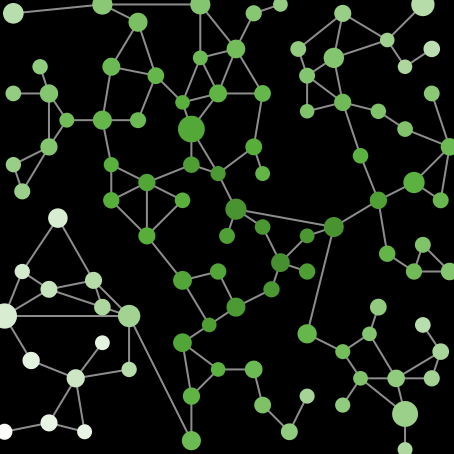
\includegraphics[width=0.49\textwidth]{figures/setup_stylized.png}\hspace{0.1cm}
	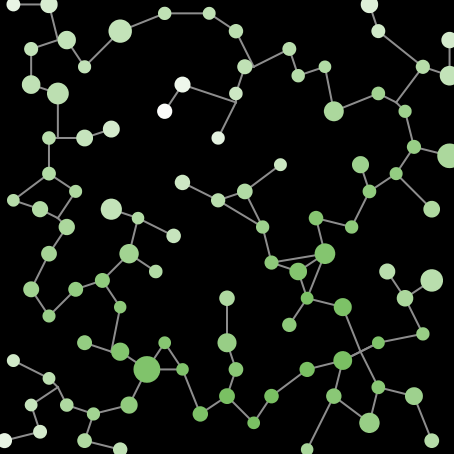
\includegraphics[width=0.49\textwidth]{figures/setup_synth_0.png}\\\vspace{0.1cm}
	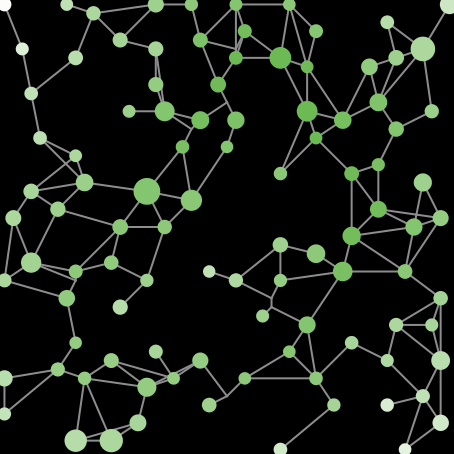
\includegraphics[width=0.49\textwidth]{figures/setup_synth_1.png}\hspace{0.1cm}
	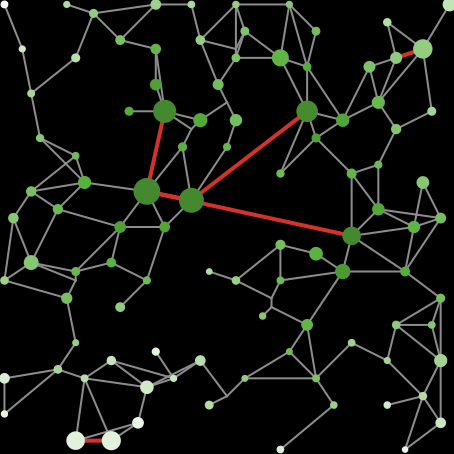
\includegraphics[width=0.49\textwidth]{figures/setup_synth_1_tick100.png}
	\caption{\textbf{Examples of model setup.} (\textit{Top Left}) Unique stylized setup provided in the initial implementation of the model \cite{schmitt2014modelisation}; (\textit{Top Right})}
\end{figure}
%%%%%%%%%%%



%%%%%%%%%%%%%%%%%%%%%
\subsection{Indicators for trajectories of systems of cities}

\subsubsection{Context}

A crucial aspect of the study of simulation models is the definition of relevant indicators, particularly in the case of synthetic models where it is not possible to produce outputs that are directly linked to data for example. Very general stylized facts, as aiming at producing an urban hierarchy or a network hierarchy, are relatively limited. Moreover, the hierarchy is mechanically produced by most models including aggregation processes. We therefore need more elaborated indicators to understand the dynamics of the system. These indicators must in particular give elements of answer to the following questions:
\begin{itemize}
	\item types of systems of cities produced by the model;
	\item change in time of the organization of the system of cities;
	\item typical profiles of trajectories;
	\item ability to ``produce some co-evolution''.
\end{itemize}


In order to concentrate on the ability of the model to produce trajectories that are both diverse and complex, and for example its ability to produce bifurcations that would manifest as inversions in ranks, and also its ability to capture different aspects of co-evolutive dynamics, we propose a set of indicators, including for example lagged correlation measures in the spirit of causality regimes introduced by~\cite{raimbault2017identification}, or a correlation measure as a function of distance, to understand the role of spatial interactions in the coupling of trajectories. Given a variable $X_i(t)$ defined for each city and in time (that will be the population or centrality measures for example), we define the following indicators.

\subsubsection{Indicators}

\paragraph{Summary statistics}

Simple but crucial indicators characterize the distribution of $X_i$ in time:
\begin{itemize}
	\item hierarchy (slope of the least squares adjustment of $X_i$ as a function of rank) $\alpha (t)$
	\item entropy of the distribution $\varepsilon (t)$
	\item descriptive statistics (average $\hat{\Eb{X}} (t)$ and standard deviation $\hat{\sigma} (t)$)
\end{itemize}


\paragraph{Rank correlation}

The rank correlation between the initial time and the final time, which translates the quantity of change in the hierarchy during the evolution of the system, and is defined by

\begin{equation}
\rho_r = \hat{\rho}\left[rg(X_i(t=0)),rg(X_i(t=t_f))\right]
\end{equation}

where $rg(X_i)$ is the rank of $X_i$ among all values (similar to a Spearman rank correlation).


\paragraph{Diversity of trajectories}

The diversity of trajectories $\mathcal{D}\left[X_i\right]$ captures a diversity of time series profiles for the considered variable. With $\tilde{X}_i(t)\in \left[0;1\right]$ the trajectories that have been individually rescaled, it is defined by

\begin{equation}
\mathcal{D}\left[X_i\right] = \frac{2}{N\cdot(N-1)}\sum_{i<j} \left(\frac{1}{T}\int_{t} \left(\tilde{X}_i(t) - \tilde{X}_j(t)\right)^2 \right)^{\frac{1}{2}}
\end{equation}

The L2-norm can be generalized by any Minkovski distance, as done in~\cite{raimbault2016hybrid}. More elaborated indices for this aspect could imply the use of specific time-series clustering techniques~\cite{liao2005clustering}.


\paragraph{Shape of trajectories}

We quantify the shape of temporal trajectories through the changes in direction of these $\mathcal{C}\left[X_i\right]$, that we take as the number of inflexion points, detected by a change of sign of the second derivative. % TODO check what is exactly implemented
In the context of such a type of model, which mainly produces monotonous trajectories, this indicator witnesses in a certain way of a ``complexity'' of trajectories. In the case of more elaborated shapes, measures such as permutation entropy would be better candidates \cite{scarpino2017predictability}.
	
	
\paragraph{Distance correlations}

Correlations as a function of distance, to understand the way the effect of distance is translated at the macroscopic scale. The profile of this function, regarding interaction distance parameters included in the model, will translate the tendency of the model to lead to the emergence of one level of interaction or the other. It is computed as

\begin{equation}
\rho_d = \hat{\rho}\left[(X(\vec{x}_k,Y(\vec{x}_{k'}))\right]
\end{equation}

where $X_i, Y_i$ are the two variables considered and $(k,k')$ the set of couples such that $\norm{\vec{x}_k-\vec{x}_{k'}} - d \leq \varepsilon$ with $\varepsilon$ a tolerance threshold (in practice taken to regroup couples by distance deciles).


\paragraph{Lagged correlations}

Lagged correlations between the variations of variables, to identify causality patterns between variables $X$ and $Y$. The patterns $\hat{\rho}_{\tau}$ for all variables, and for $\tau$ lag or anticipation, must be understood in the sense of potential regimes, explored by \cite{raimbault2017identification}.

\begin{equation}
\rho_{\tau} = \hat{\rho}\left[\Delta X(t-\tau),\Delta Y(t)\right]
\end{equation}



We furthermore introduce diverse indicators for network topology, to understand the final forms produced by the heuristic: diameter, average path length, average betweenness centrality and its level of hierarchy, average performance, total length, as they have been defined to quantify urban form in~\cite{2018arXiv180505195R}.
% TODO not needed as not described in results


\subsubsection{Variables}


These indicators are used in our case on the following variables:
\begin{itemize}
	\item populations $\mu_i(t)$,
	\item closeness centralities
	\[c_i(t) = \frac{1}{N-1}\sum_{i\neq j} \frac{1}{d_{ij}(t)}\]
	which capture the position within the urban system,
	\item accessibilities \[X_i = \frac{1}{\sum_k \mu_k}\sum_{i\neq j} P_j \exp{\left(- d_{ij}(t)/d_G\right)}\] which capture the insertion within the urban system.
\end{itemize}

They capture both city trajectories, network trajectories, and the coupling of both with accessibility.



%%%%%%%%%%%%%%%%%
\section{Results}
%%%%%%%%%%%%%%%%%


%%%%%%%%%%%%%%%
\subsection{Model implementation}

We modified and extended the NetLogo implementation of the model provided by \cite{schmitt2014modelisation}, to include in particular (i) methods for the synthetic setup; (ii) indicators described above; (iii) methods for the inclusion within OpenMOLE experiments. The modified code with exploration scripts are available on the open git repository of the project at \url{https://github.com/JusteRaimbault/CityNetwork/tree/master/Models/Reproduction/SimpopNet}.



%%%%%%%%%%%%%%%
\subsection{Experience plan}

Given an initial spatial configuration (i.e. a value of meta-parameters), we establish the behavior of indicators by exploring a grid of the parameter space. The number of parameters being low and the objective being a first grasp of the model behavior, in particular if it is able to produce co-evolution dynamics, we do not use more elaborated exploration methods. The parameters are $(d_G,\gamma_G,\gamma_N,\theta_N,v_0)$ and meta-parameters $(N_S,\alpha_S,d_S,n_S)$. We take also the meta-parameters into account in order to understand the sensitivity of the model to space.


We explore a grid of 16 configurations of meta-parameters, 324 configurations of parameters, and 30 random replications, what corresponds to $155520$ simulations. They are executed on a computation grid with the intermediary of OpenMole. Simulation results are available at \url{http://dx.doi.org/10.7910/DVN/RW8S36}.


%%%%%%%%%%%%%%%%%%%%%%
\subsection{Convergence}

Since the model is stochastic, it is important to control the convergence of indicators, that will be more or less easy depending on their variability. To quantify the variability of an indicator $X$ regarding stochasticity, we use a measure similar to the one used by~\cite{raimbault2018calibration}, given by $v\left[X\right] = \hat{\mathbb{E}}\left[X\right]/\hat{\sigma}\left[X\right]$ with basic estimators for the expectancy and the standard deviation. On the full set of replications, we obtain for all indicators given previously, a median for the ratio $v\left[X\right]$ estimated within replications, estimated on all parameter values, which takes a minimal value of $3.94$, for the average accessibility at final time, what witnesses a low stochastic variability. We can furthermore use this value to estimate the level of convergence: it corresponds to a 95\% confidence interval around the mean of relative size $0.18$ (under the assumption of a normal distribution of the average), i.e. a good convergence. This aspect is crucial for the robustness of results.


%%%%%%%%%%%%%%%%%%%%%%
\subsection{Sensitivity to space}

The Table~\ref{tab:macrocoevolexplo:spacematters} give values of $\tilde{d}$ for 16 configurations of meta-parameters. The definition of the relative measure of sensitivity, given by~\cite{cottineau2017initial}, is for two phase diagrams $f_1,f_2$ and $d$ euclidian distance, 

\begin{equation}
\tilde{d} = 2 d(f_1,f_2)/(\Varb{f_1}+\Varb{f_2})
\end{equation}

These are given in comparison to an arbitrary reference configuration (first column). The hierarchy within the initial system of cities appears as the stronger determinant of variability, since all configurations with $\alpha_S = 1.5$ give values larger than $1.7$, what witnesses a very strong sensitivity relative to this hierarchy.

Then, the number of cities plays a non negligible secondary role , giving the stronger effects of space. Thus, it is crucial to keep in mind this role of the initial configuration during the analysis of phase diagrams. To stay within the same spirit than the model that was initially proposed, we will however comment a phase diagram for a given spatial configuration. The study of the extended model with integration of meta-parameters to which it is sensitive at their full extent is beyond the reach of this auxiliary analysis.





%%%%%%%%%%%%%
\begin{table}[!ht]
\caption{\textbf{Sensitivity to space of the SimpopNet model.} Each column corresponds to an instance of the phase diagram, for which meta-parameters are given, with the relative distance to an arbitrary reference diagram. As inputs we have the meta-parameters $N_S,\alpha_S,d_S,n_S$ and as outputs of simulations the distance $\tilde{d}$.\label{tab:macrocoevolexplo:spacematters}}
\centering
\begin{tabular}{|l|l|l|l|l|l|l|l|l|l|l|l|l|l|l|l|l|}
\hline
$N_S$ & 40 & 40 & 40 & 40 & 40 & 40 & 40 & 40 & 80 & 80 & 80 & 80 & 80 & 80 & 80 & 80\\
$\alpha_S$ & 0.5 & 0.5 & 0.5 & 0.5 & 1.5 & 1.5 & 1.5 & 1.5 & 0.5 & 0.5 & 0.5 & 0.5 & 1.5 & 1.5 & 1.5 & 1.5\\
$d_S$ & 5 & 5 & 10 & 10 & 5 & 5 & 10 & 10 & 5 & 5 & 10 & 10 & 5 & 5 & 10 & 10\\
$n_S$ & 10 & 30 & 10 & 30 & 10 & 30 & 10 & 30 & 10 & 30 & 10 & 30 & 10 & 30 & 10 & 30\\\hline
$\tilde{d}$ & 0 & 0.05 & 0.26 & 0.21 & 1.79 & 1.80 & 1.79 & 1.72 & 0.44 & 0.36 & 0.42 & 0.42 & 2.25 & 2.23 & 2.24 & 2.21\\\hline
\end{tabular}
\end{table}
%%%%%%%%%%%%%


%%%%%%%%%%%%%%%%%%%%%%%%%%
\subsection{Model behavior}

The Fig.~\ref{fig:macrocoevolexplo:behavior} reports the behavior of the model according to a selection among the diverse indicators given above. We comment a particular spatial configuration which corresponds to a low hierarchical system with a network having only local shortcuts, given by meta-parameters $N_S=80,\alpha_S=0.5,d_S=10,n_S=30$, which are the values giving configurations that are the most similar to the one of the initial model. More exhaustive plots for this parameter configuration are available in~\cite{raimbault:tel-01857741} (Appendix A.7).


The values taken by the entropy for centralities (first panel of Fig.~\ref{fig:macrocoevolexplo:behavior}), as a function of time, for $\gamma_N = 2.5$ and $v_0 = 110$, exhibit different regimes depending on $d_G$ and $\gamma_G$. A low hierarchy leads to an entropy stabilizing in time, what corresponds to a certain uniformization of distances. On the contrary, a strong hierarchy produces a regime with a minimum, and then an increase of disparities in time.


This variety of behaviors can be found again with the rank correlation $\rho_R$, that we show here for the population variable, as a function of $d_G$. It has a low sensitivity to $\theta_N$ and $\gamma_N$ (see~\cite{raimbault:tel-01857741}, Appendix A.7), but strongly varies as a function of $d_G$ and $\gamma_G$: interactions at a higher distance induce systematically a larger number of changes in the hierarchy of populations. These can occur when the hierarchy of distance is low. To summarize, the increase of the range of interactions will diminish the inertia of trajectories of the system of cities, whereas the increase of their hierarchy will increase it. This is relatively credible from a thematic point of view: longer and uniform interactions have more chances to make individual trajectories change.




%%%%%%%%%%%%%%%%
\begin{figure}
	%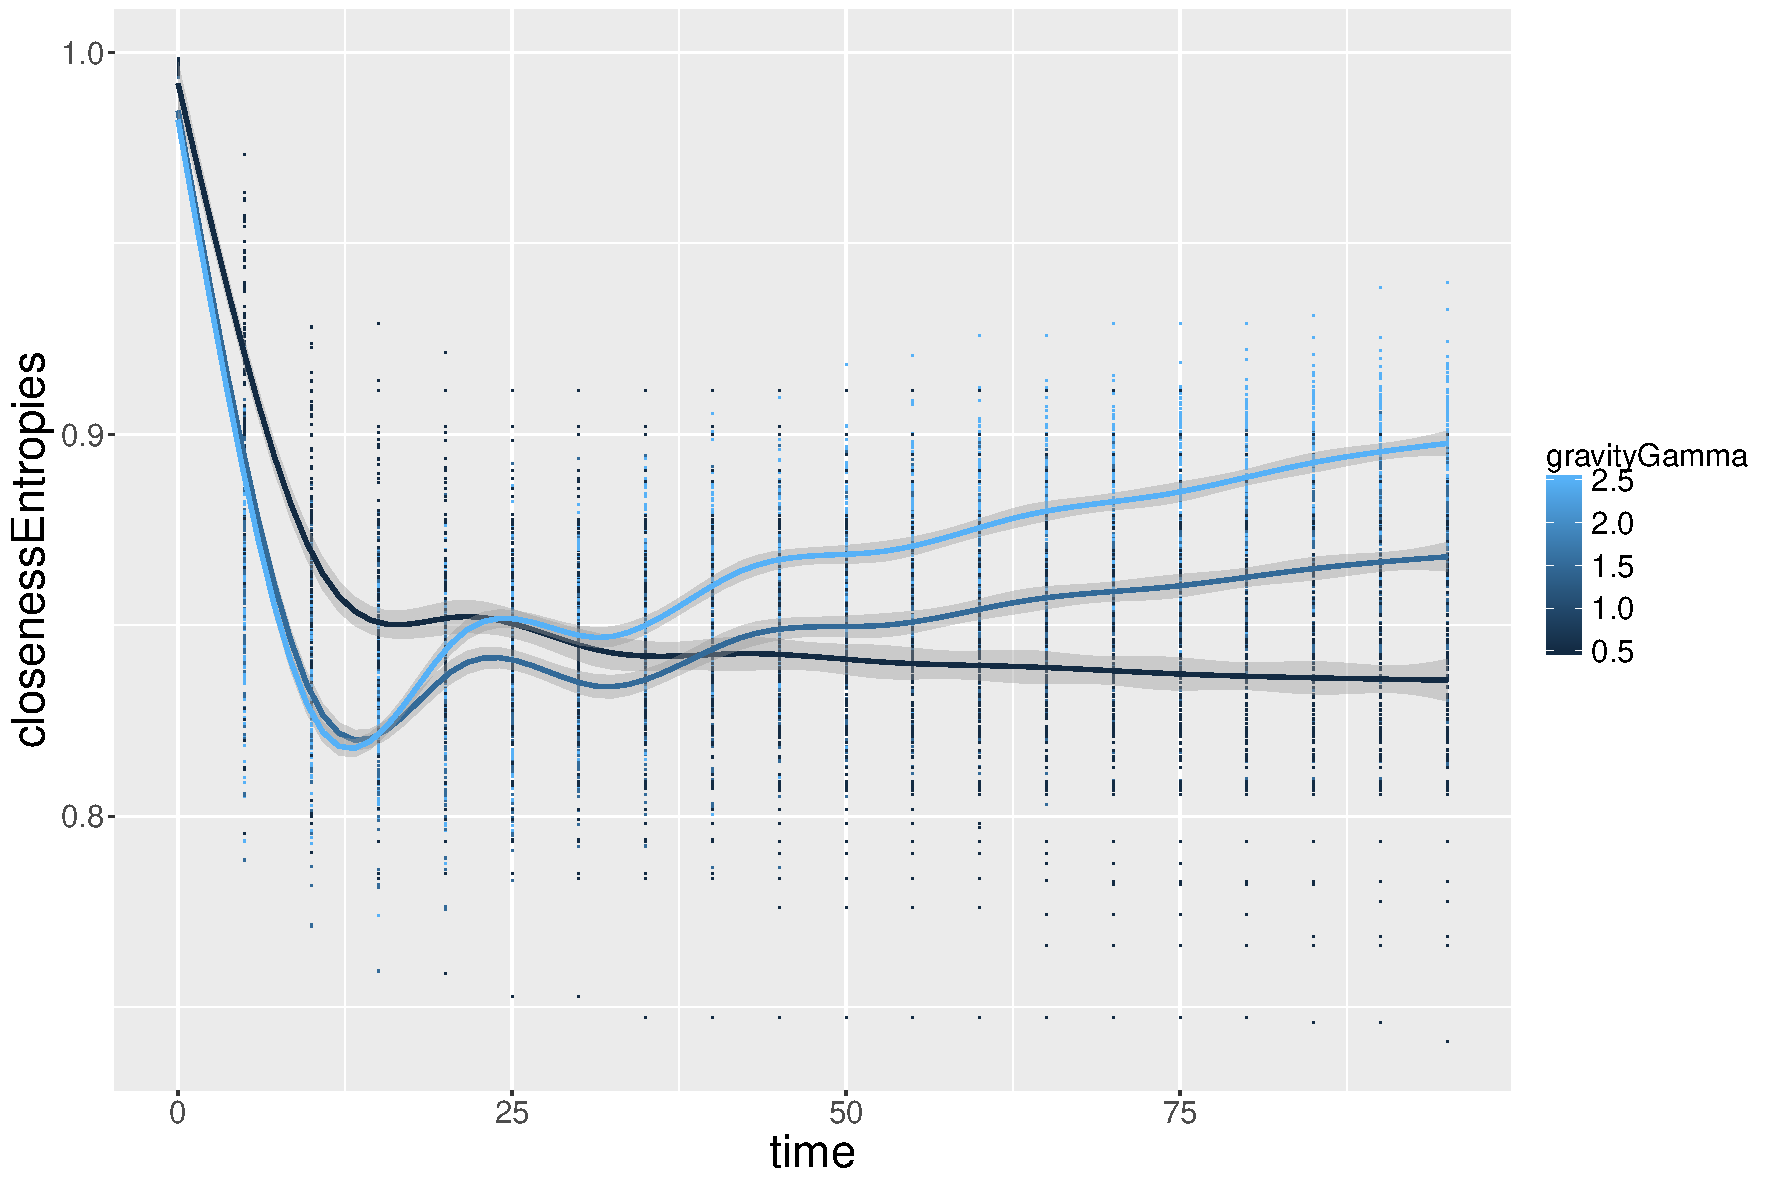
\includegraphics[width=0.48\linewidth]{Figures/MacroCoEvolExplo/closenessEntropies_networkGamma2.5_networkSpeed110_gravityDecay0.016_networkThreshold11.pdf}
	%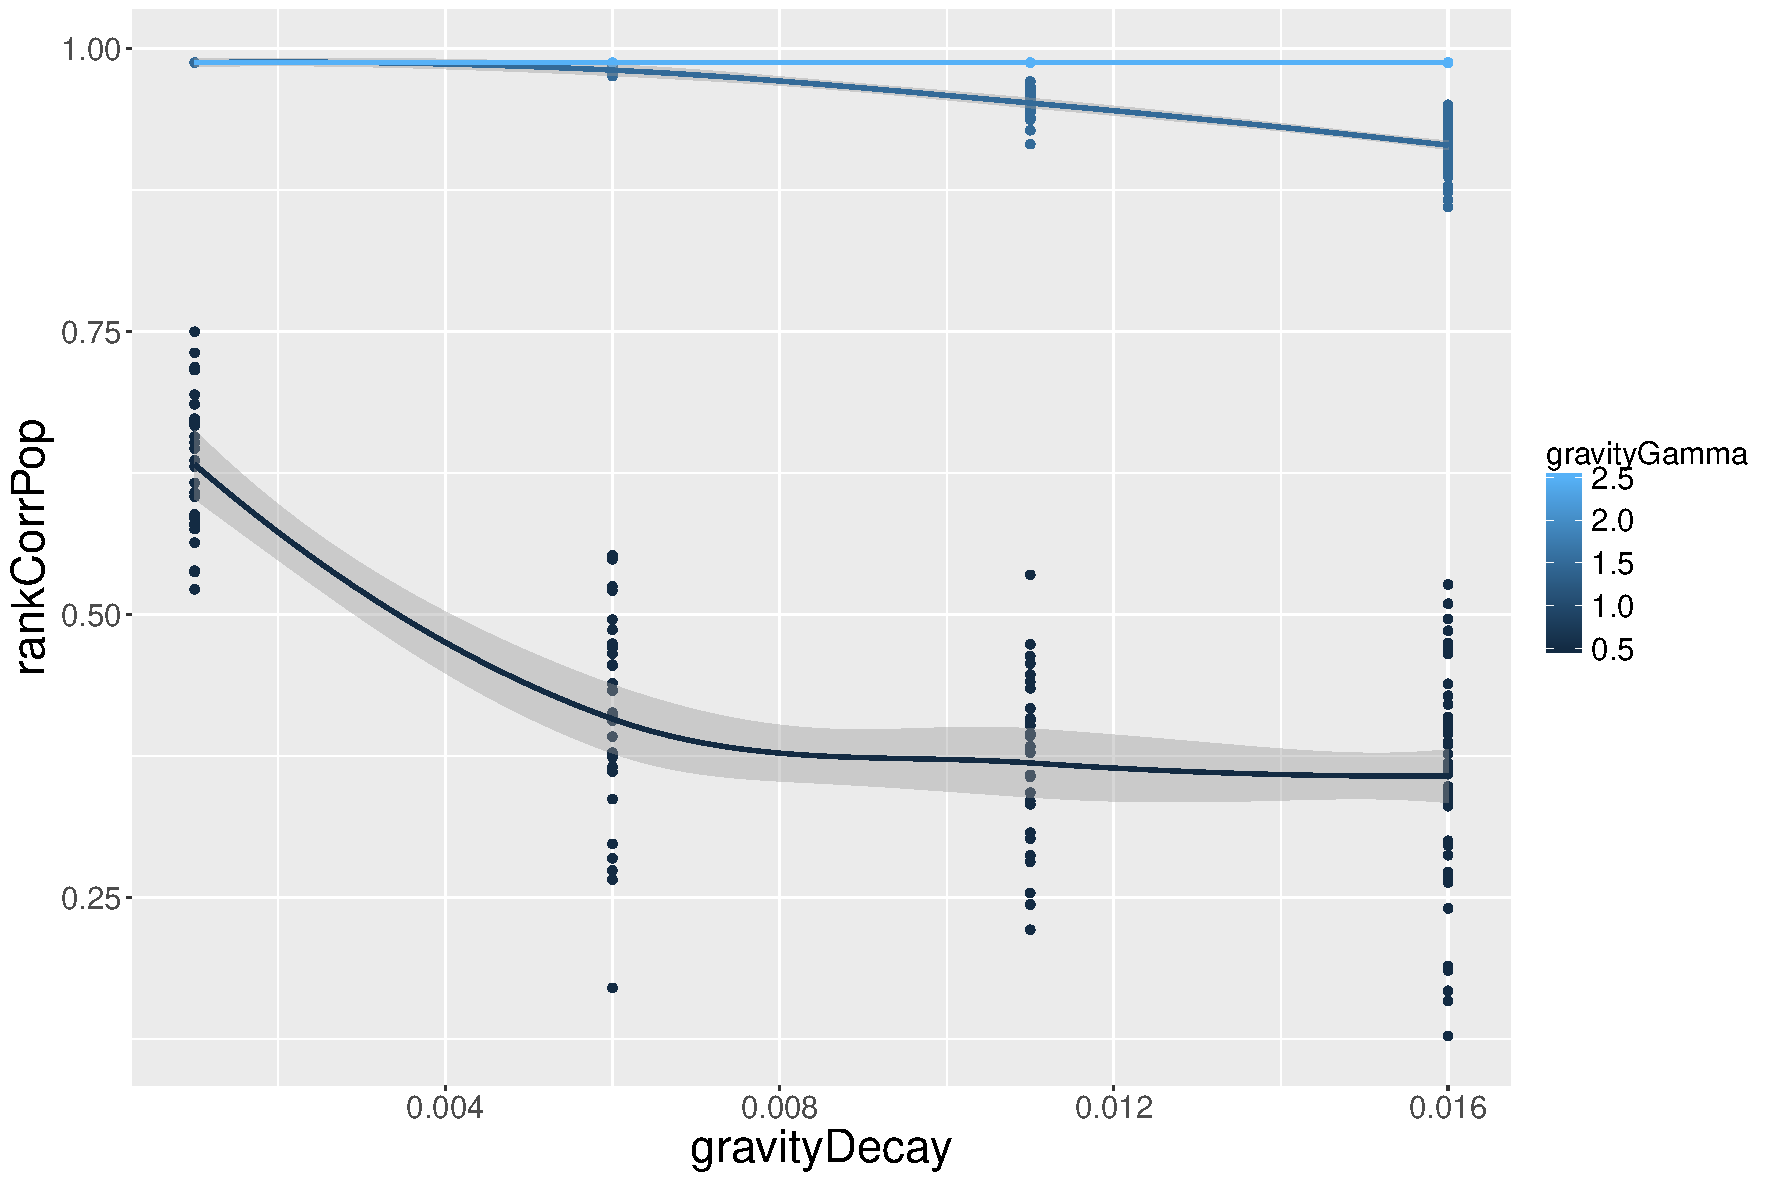
\includegraphics[width=0.48\linewidth]{Figures/MacroCoEvolExplo/rankCorrPop_networkSpeed110_networkThreshold11_networkGamma2.5.pdf}\\
	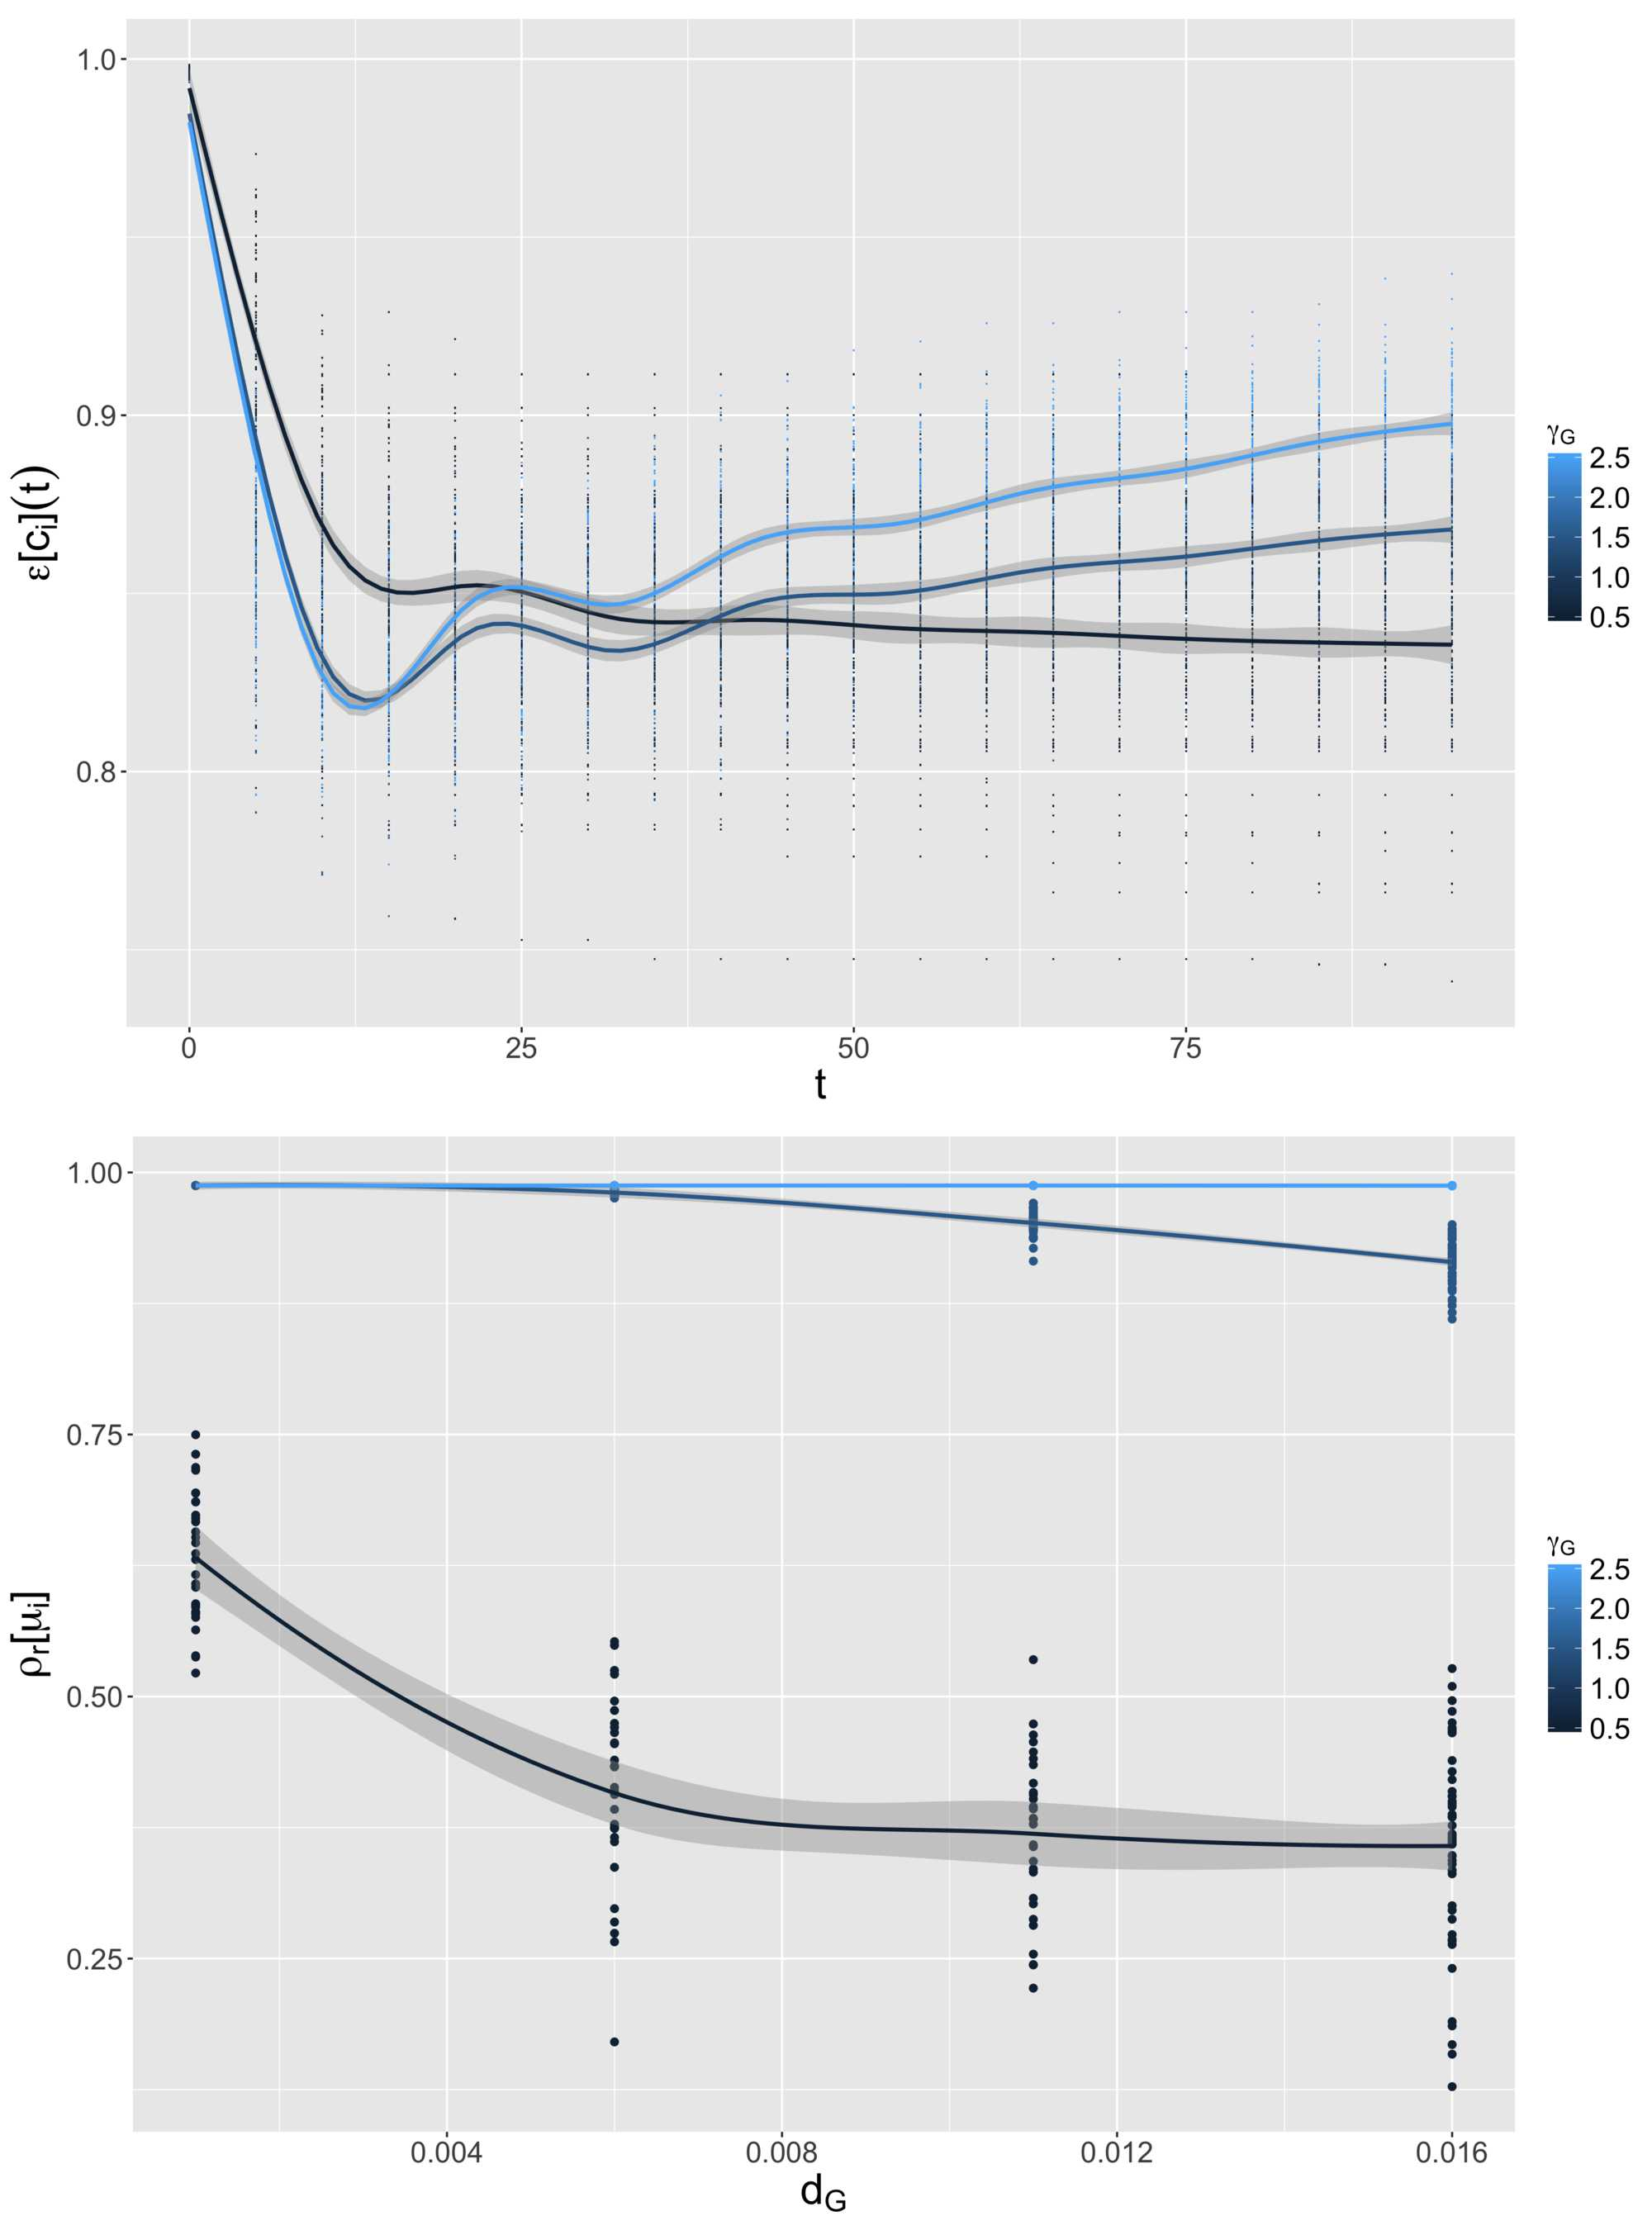
\includegraphics[width=\linewidth,height=0.85\textheight]{figures/6-1-3-fig-macrocoevolexplo-behavior.jpg}
	\caption{\textbf{Model behavior for the spatial configuration $N_S=80,\alpha_S=0.5,d_S=10,n_S=30$.} (\textit{Top}) Temporal trajectories of the entropy for closeness centralities, for $\gamma_N = 2.5$, $v_0 = 110$, $d_G = 0.016$, $\theta_N = 11$, as a function of $\gamma_G$ (color); (\textit{Bottom}) Rank correlation for population, as a function of $d_G$ and of $\gamma_G$ (color), for $\theta_N = 11$, $\gamma_N = 2.5$.\label{fig:macrocoevolexplo:behavior}}
\end{figure}
%%%%%%%%%%%%%%%%


The behavior of correlation indicators is shown in Fig.~\ref{fig:macrocoevolexplo:correlations}. Concerning the effect of distance on correlations between variables, i.e. the evolution of $\rho_d$, it is interesting to note that an increase of $d_G$ systematically diminishes the levels of correlation, what corresponds to the complexification that we previously showed. As expected, $\rho_d\left[d\right]$ decreases as a function of distance, and exhibits non zero values for the correlation between population and centrality for a high hierarchy $\gamma_G$, what shows that simultaneous adaptation regimes are rare in this model.


%%%%%%%%%%%%%%%%%%%%%%%%%%%%%
\subsection{Causality regimes}


Finally, by studying $\rho_{\tau}$ (Fig.~\ref{fig:macrocoevolexplo:correlations}, bottom panel), we observe that causality regimes in the sense of~\cite{raimbault2017identification} are not very varied (see~\cite{raimbault:tel-01857741}, Appendix A.7, for the confirmation for a broader range of parameters). The population is systematically caused by the centrality, but there exists no regime in which we observe the contrary. This is a logic of an effect of reinforcement of hierarchy by centrality, but not a configuration with circular causalities, and thus not a co-evolution properly speaking as we defined in the statistical sense.



% -- positive only
%unique(signs$sign)
%[1] "00/00/00" "00/00/10" "01/00/10" "00/10/00" "01/00/00"


%  -- with negative --
% unique(signs$sign)
% [1] "-1-1/00/00"     "-1-1/00/-10"    "-1-1/00/10"     "-10/00/00"      "-10/00/10"      "01/00/10"      
% [7] "00/00/10"       "-11/00/10"      "-1-1/-10/-10"   "-1-1/-1-1/-10"  "-1-1/-10/-1-1"  "-1-1/-1-1/-1-1"
% [13] "-1-1/10/-10"    "-1-1/-1-1/00"   "00/00/00"       "0-1/00/00"      "01/00/00"       "-1-1/-10/00"   
% [19] "01/00/-10"      "-1-1/1-1/-10" 



%%%%%%%%%%%%%%%%
\begin{figure}
	%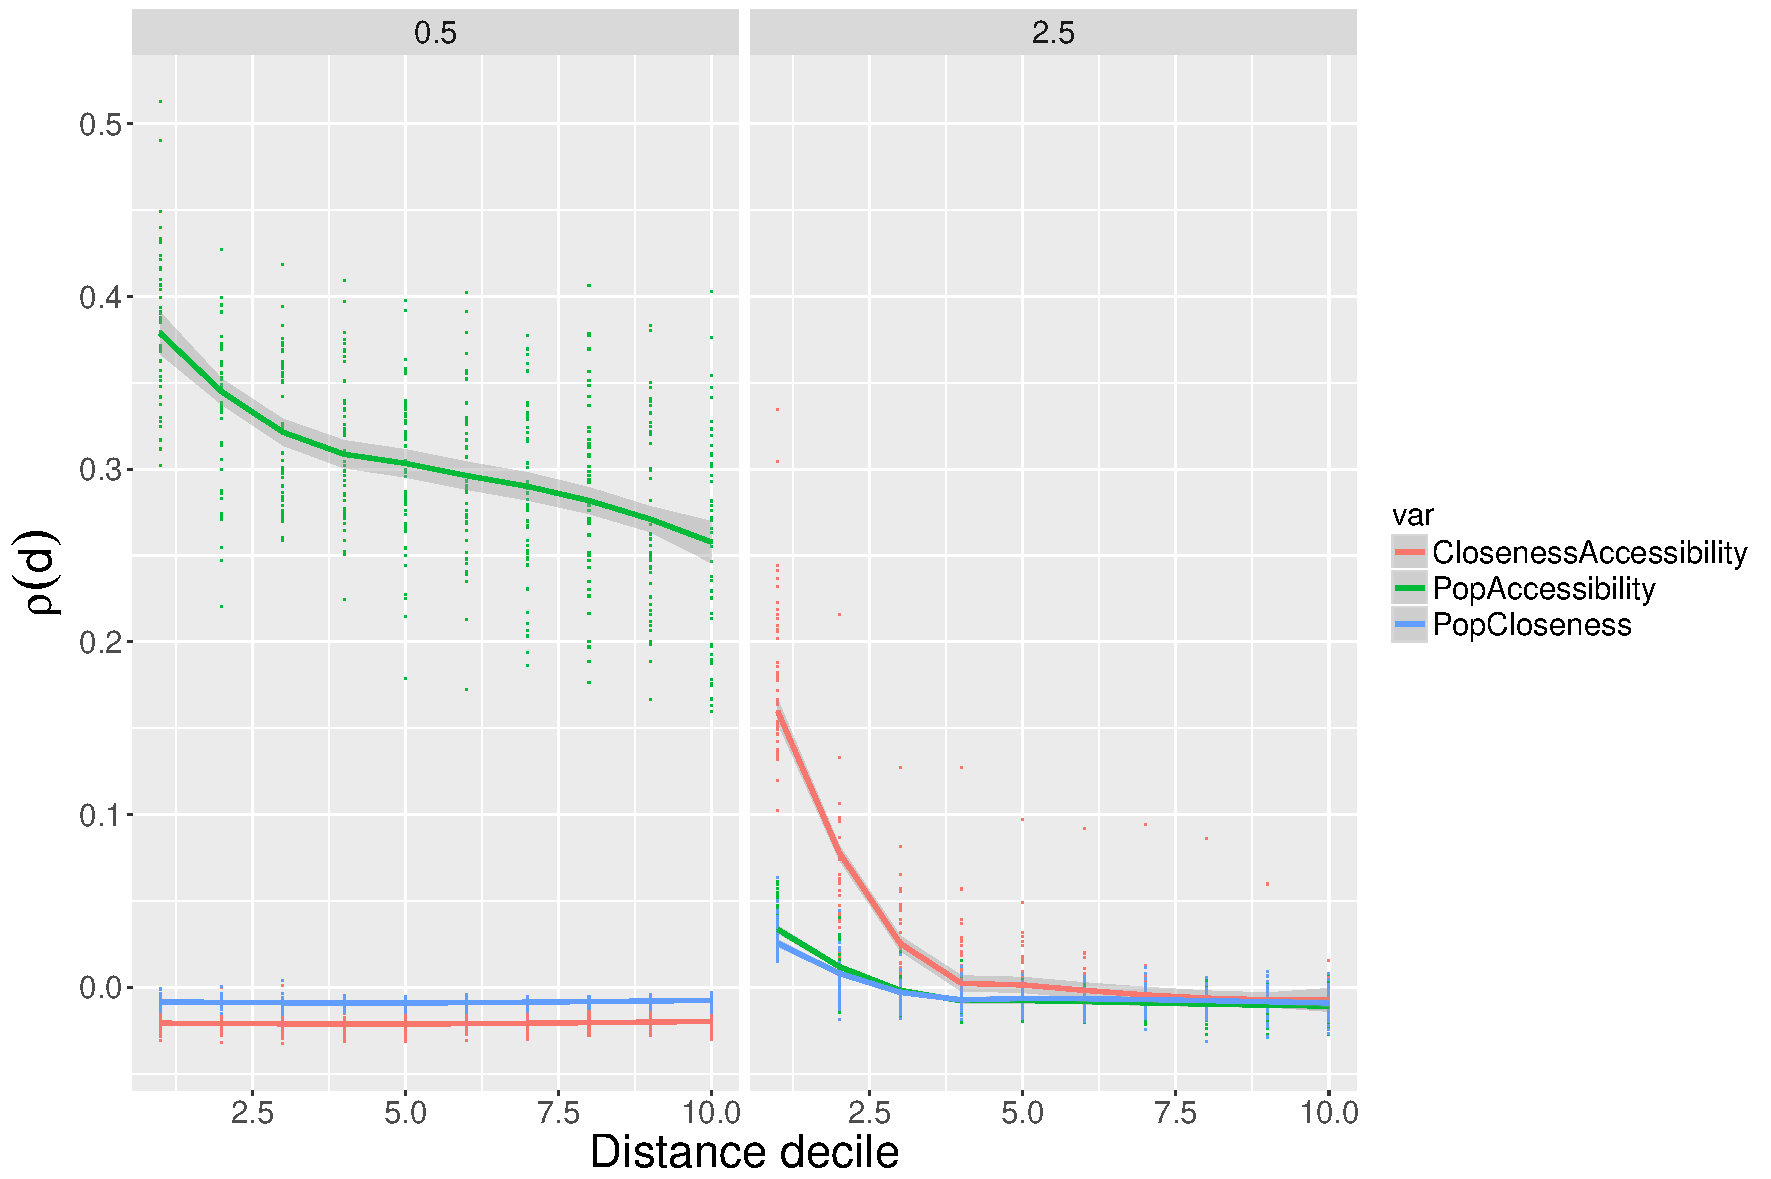
\includegraphics[width=0.48\linewidth]{Figures/MacroCoEvolExplo/distcorrs_networkGamma2.5_networkSpeed110_gravityDecay0.016_networkThreshold11.pdf}
	%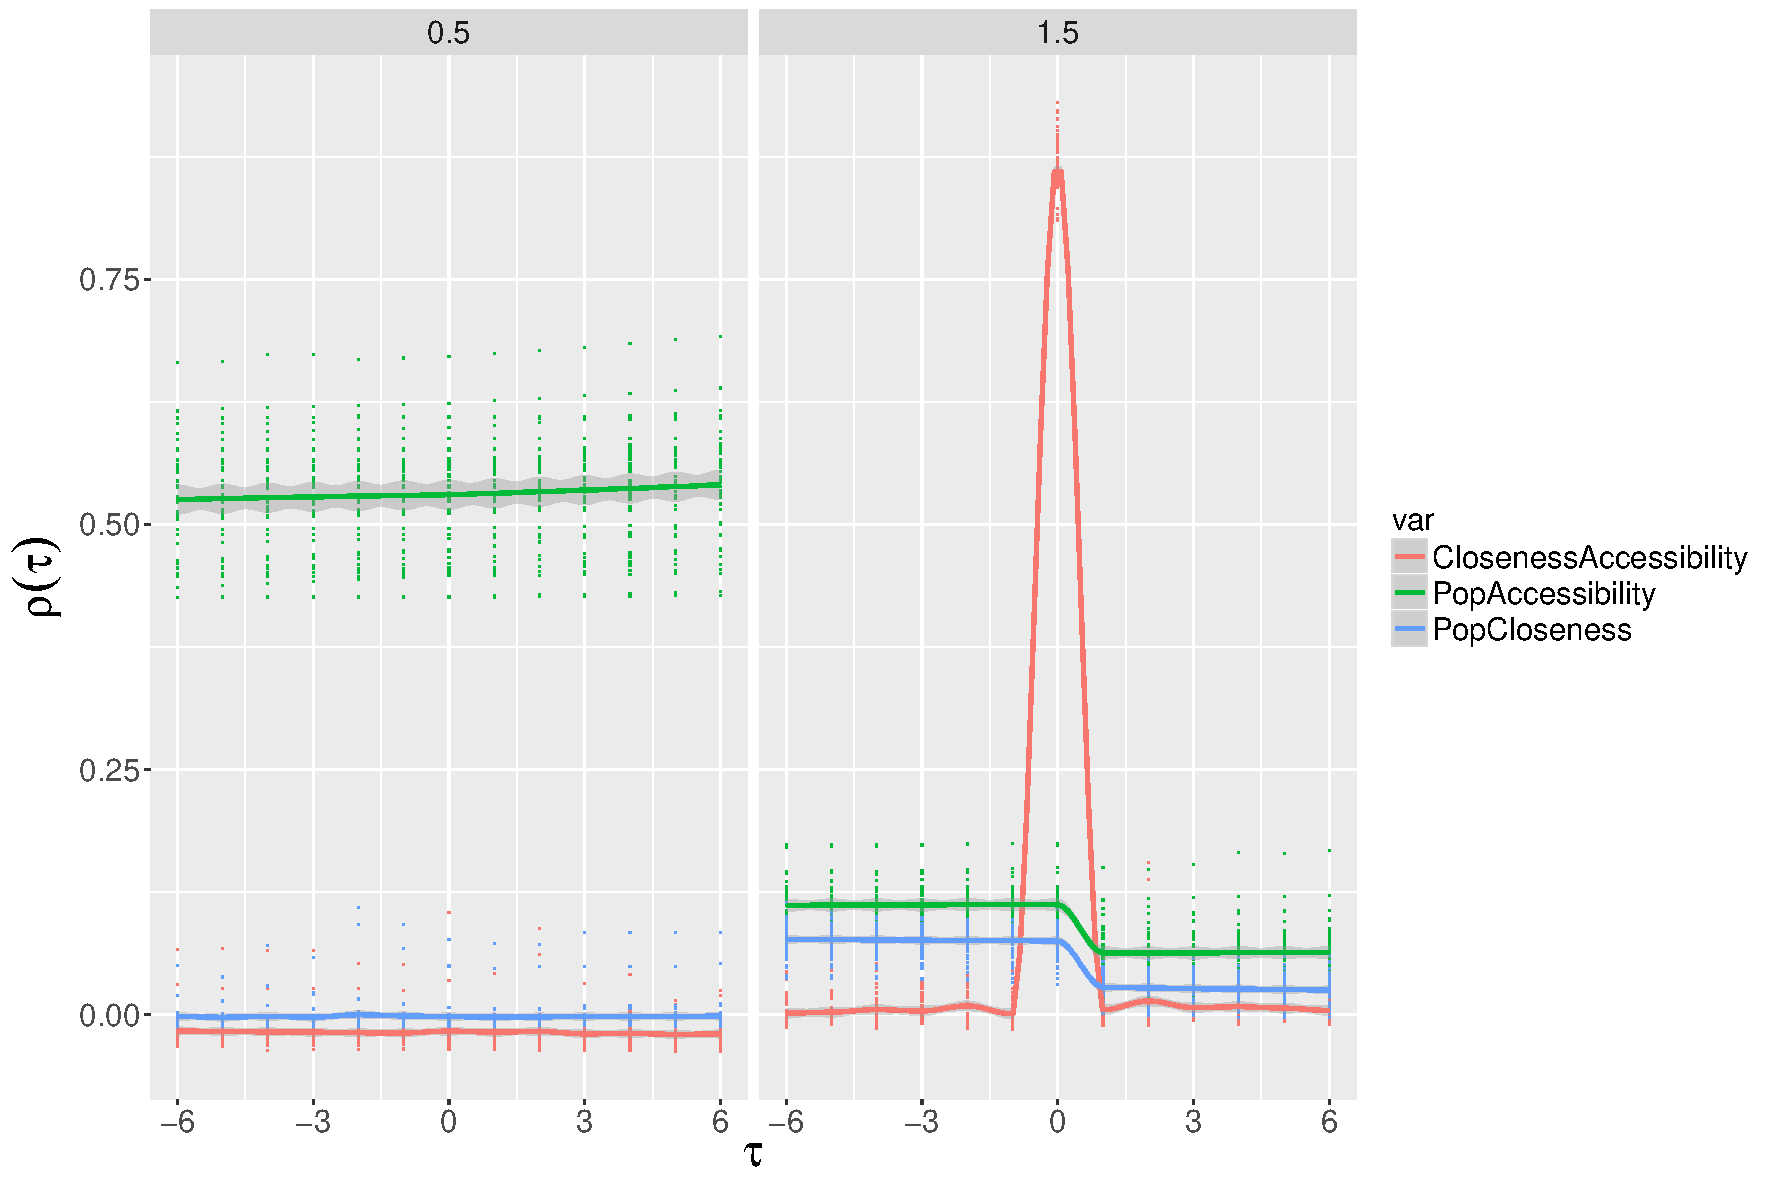
\includegraphics[width=0.48\linewidth]{Figures/MacroCoEvolExplo/laggedcorrs_networkGamma2.5_networkSpeed10_gravityDecay0.016_networkThreshold21.pdf}
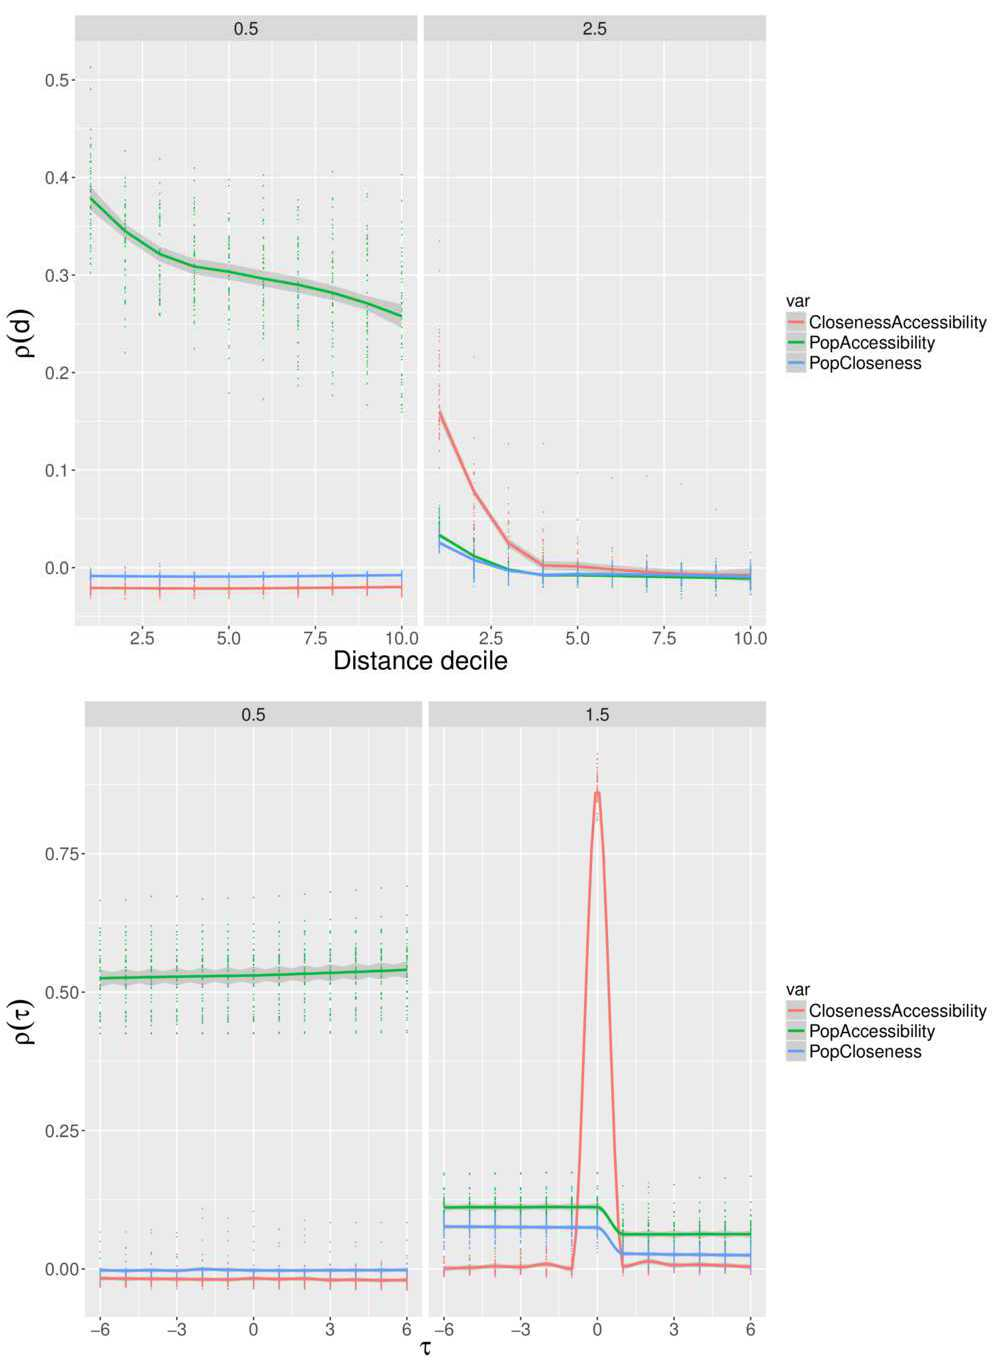
\includegraphics[width=\linewidth,height=0.9\textheight]{figures/6-1-3-fig-macrocoevolexplo-correlations.jpg}
	\caption{\textbf{Correlations in the model for the spatial configuration $N_S=80,\alpha_S=0.5,d_S=10,n_S=30$.} (\textit{Top}) Correlations as a function of distance, for couples of variables (color), for $\gamma_N = 2.5$, $\theta_N = 21$, $v_0 = 10$, and for $d_G$ (columns) and $\gamma_G$ (rows) variables; (\textit{Bottom}) Lagged correlations for the same parameters. \label{fig:macrocoevolexplo:correlations}}
\end{figure}
%%%%%%%%%%%%%%%%


This brief exploration allows us to say that this model captures urban trajectories of a certain complexity, but that it does apparently not reproduces co-evolution regimes.



%%%%%%%%%%%%%%%%%%%
\subsection{PSE algorithm}




The Fig.~\ref{fig:pse} gives the results as a scatterplot of diversity targets of the algorithm.


%%%%%%%%%%%%%%
\begin{figure}
	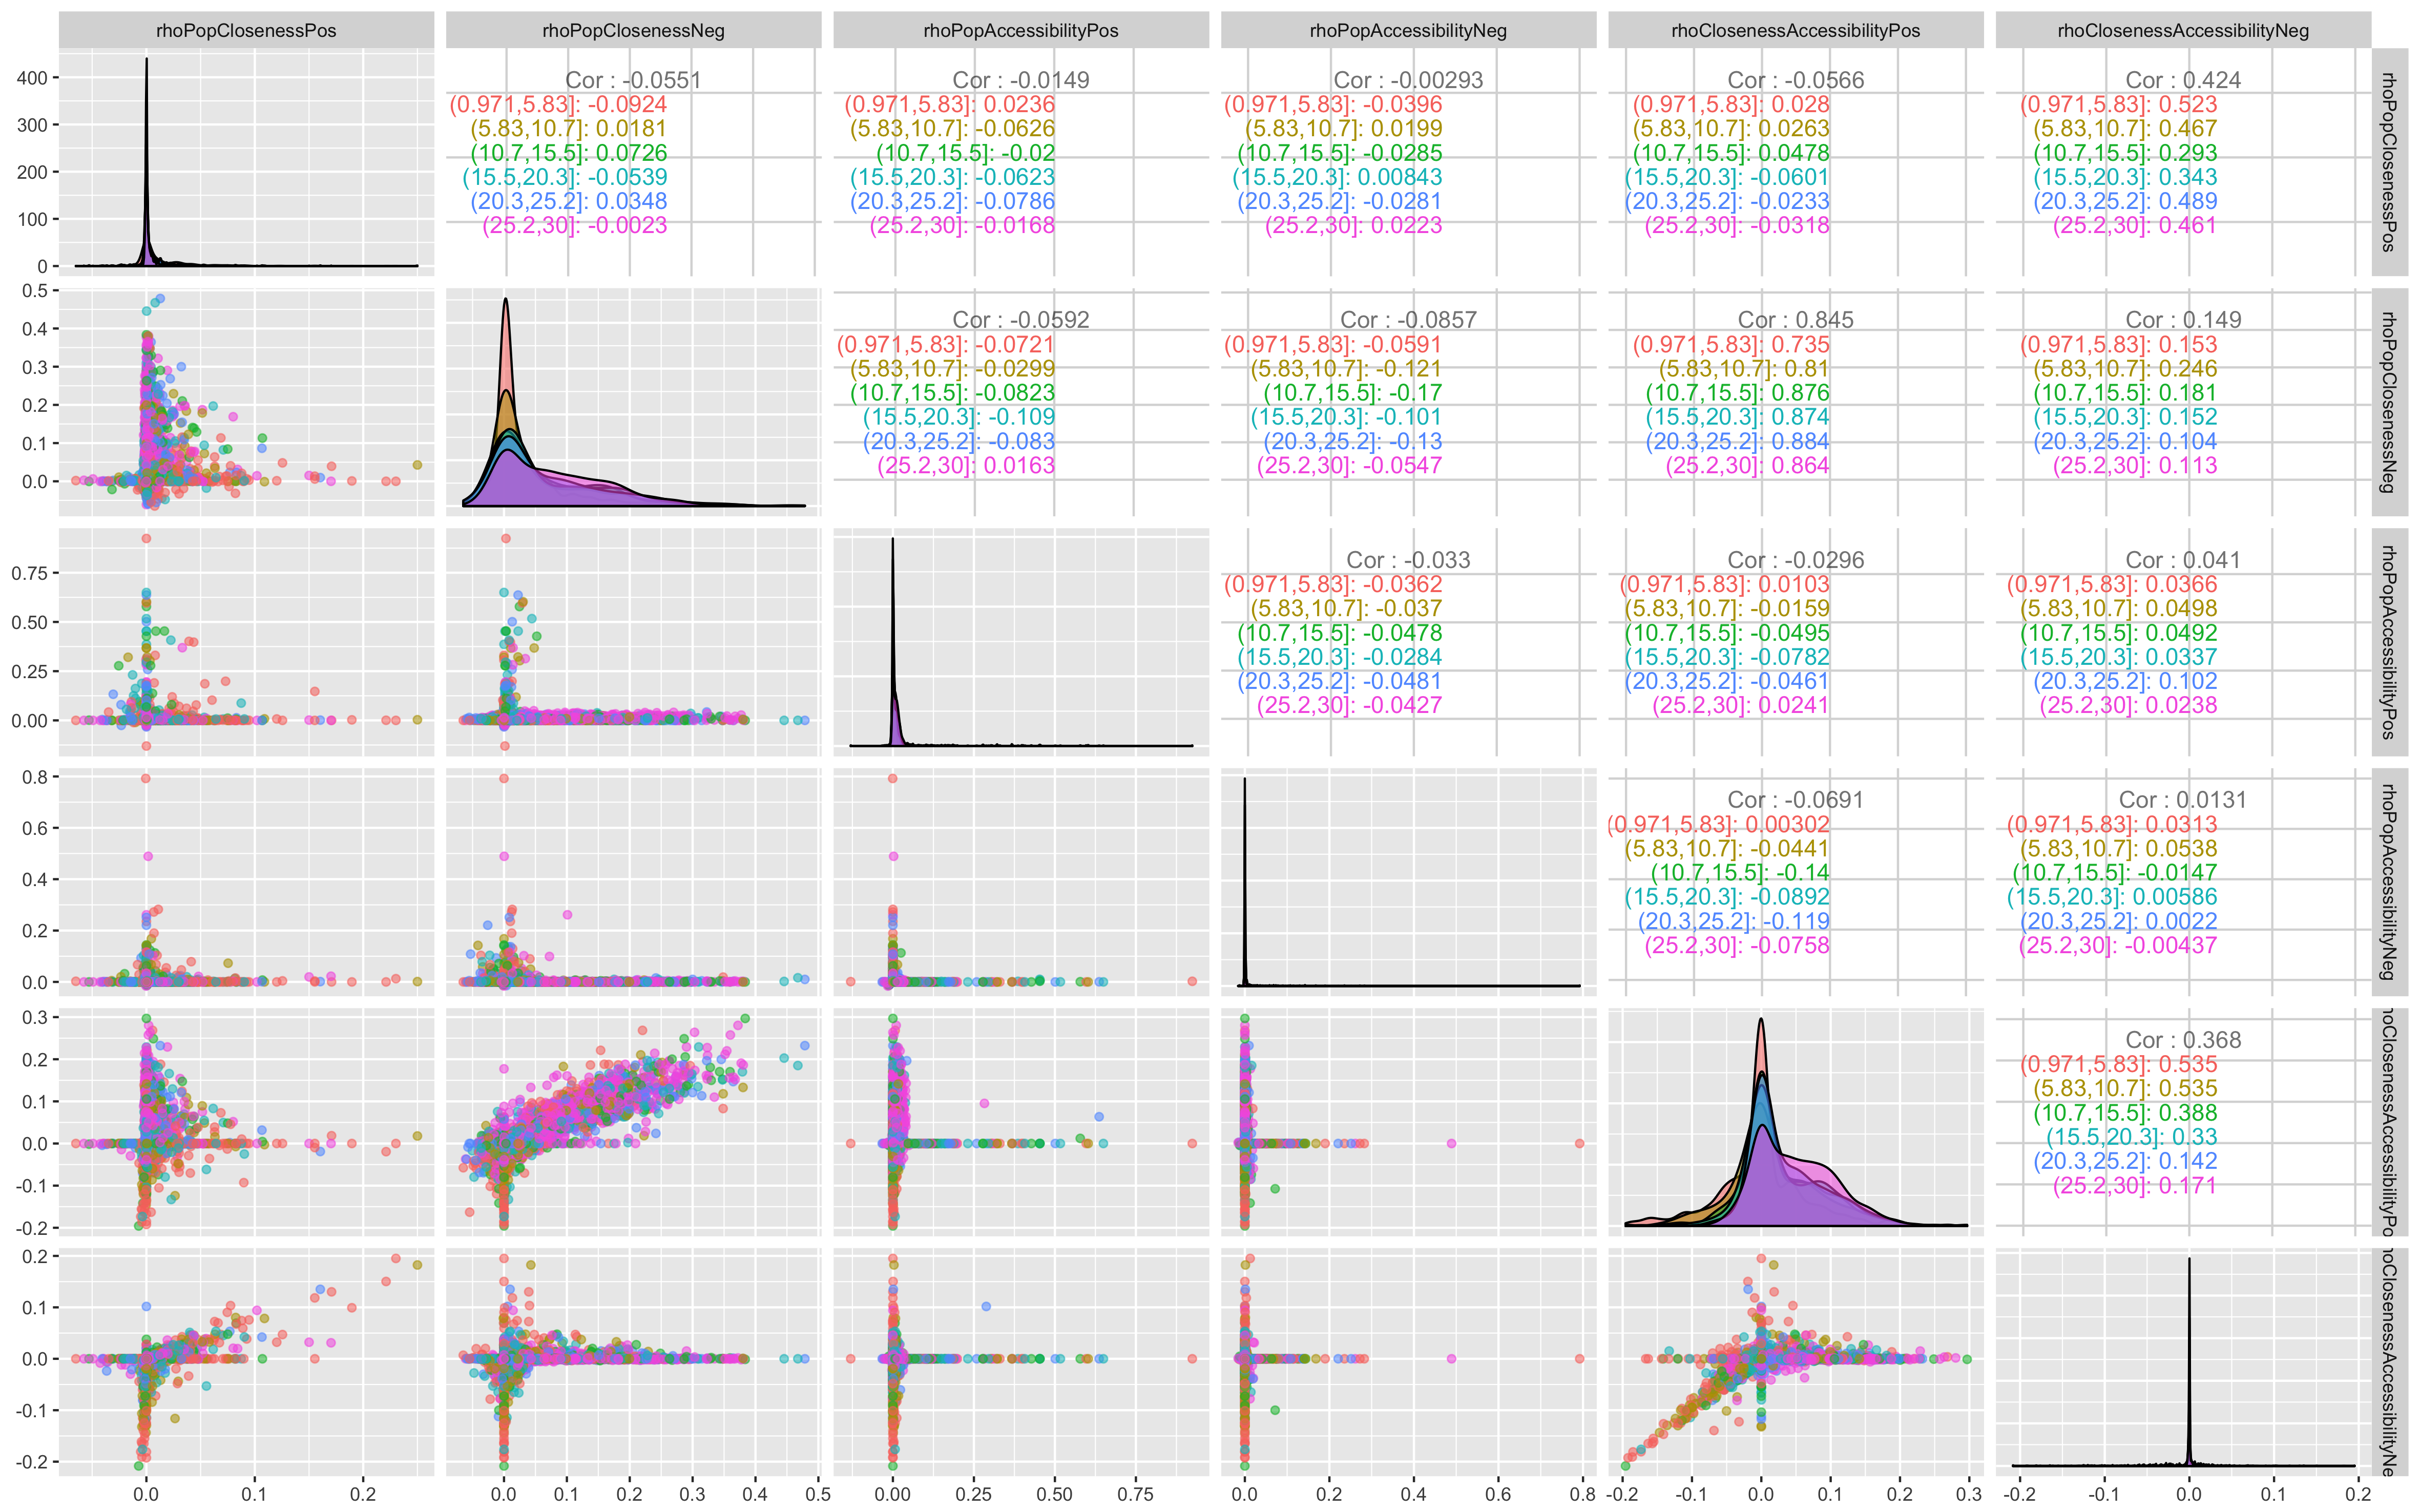
\includegraphics[width=\textwidth]{figures/scatterplot_colornwThreshold.png}
	\caption{\textbf{Feasible space of lagged correlation obtained with the PSE algorithm.}\label{fig:pse}}
\end{figure}
%%%%%%%%%%%%%%



%%%%%%%%%%%%%%%%%%%%
\section{Discussion}
%%%%%%%%%%%%%%%%%%%%


In comparison, the co-evolution model introduced by \cite{2018arXiv180409430R} is less constraints for network dynamics and produces more varied interaction regimes.




%%%%%%%%%%%%%%%%%%%%
\section{Conclusion}
%%%%%%%%%%%%%%%%%%%%


We have thus in this section introduced the tools to understand trajectories produced by a co-evolution model, and tested these on the SimpopNet model.






%
\begin{acknowledgement}
Results obtained in this paper were computed on the vo.complex-system.eu virtual organization of the European Grid Infrastructure ( http://www.egi.eu ). We thank the European Grid Infrastructure and its supporting National Grid Initiatives (France-Grilles in particular) for providing the technical support and infrastructure.
\end{acknowledgement}


%
%\section*{Appendix}
%\addcontentsline{toc}{section}{Appendix}
%

%We give here supplementary figures allowing to render the sensitivity of results to parameters not presented in main text. The Fig~\ref{fig:app:macrocoevolexplo:closeness} allows to visualize the sensitivity of the entropy of centralities $\varepsilon \left[\mu_i\right]$ as a function of $d_G$, $\theta_N$ and $\gamma_G$. The shape of temporal curves is mainly sensitive to $\gamma_G$.
%Finally, we give in Fig.~\ref{fig:app:macrocoevolexplo:laggedcorrs} the lagged correlations $\rho_{\tau}$ between all couples of variables, for varying $d_G$ and $\gamma_G$. Similarly, qualitative behaviors are globally stable for other parameters than $\gamma_G$.
%The Fig.~\ref{fig:app:macrocoevolexplo:rankcorrpop} gives the variations of $\rho_r$ as a function of $d_G$ and $\gamma_G$, for variable values of $\theta_N$ and of $\gamma_N$. We see that the regularity observed as a function of $d_G$ and of $\gamma_G$ appears not to be sensitive to the variations of $\theta_N$ and of $\gamma_N$.
%The Fig.~\ref{fig:app:macrocoevolexplo:distcorrs} gives correlations $\rho_d$ as a function of distance for all couples of variables, for varying $d_G$ and $\gamma_G$. We obtain qualitatively the same behaviors than with $d_G = 0.016$, at the exception of a very low growth for the largest distances, for the correlation between population and accessibility, at $d_G=0.001$ and $\gamma_G = 0.5$, which remains difficult to interpret.



%
%%%%%%%%%%%%%%%%%%
%\begin{figure}
%    %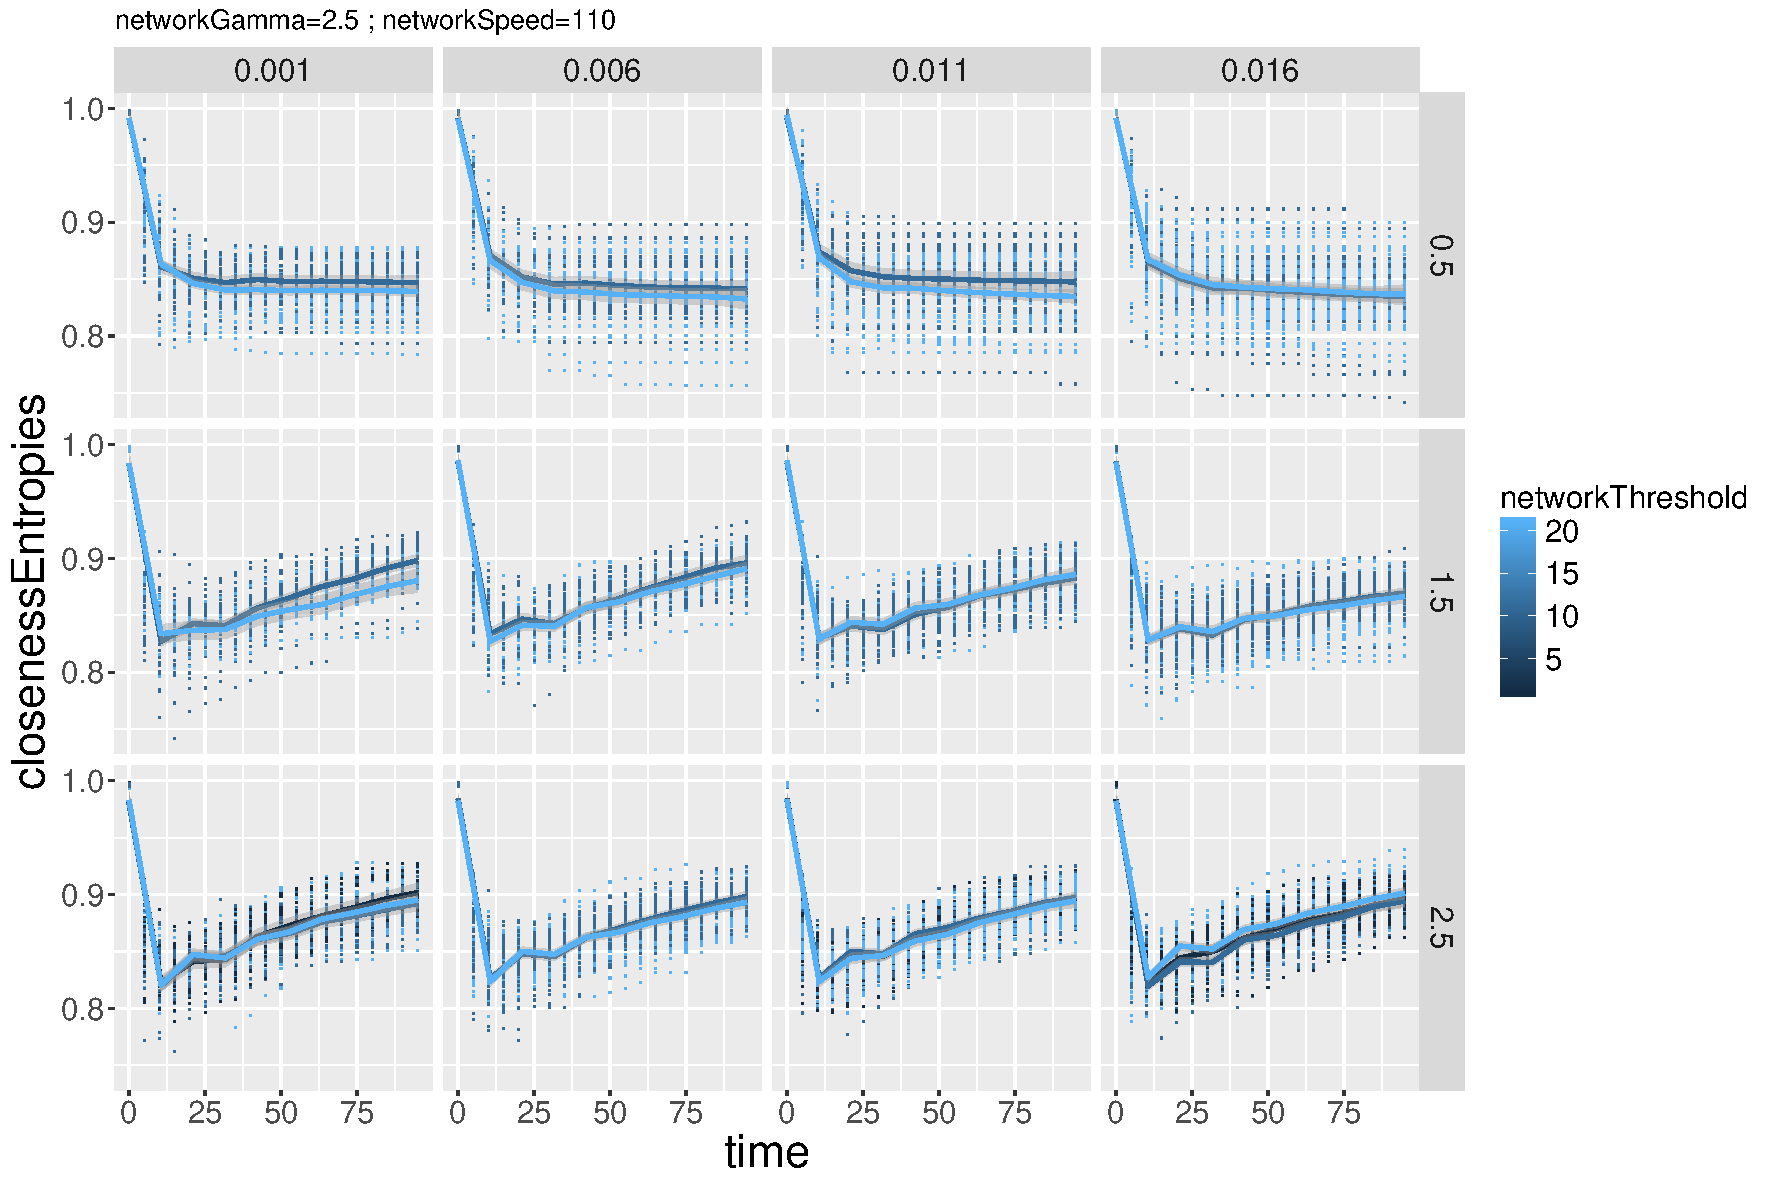
\includegraphics[width=0.48\linewidth]{Figures/MacroCoEvolExplo/closenessEntropies_networkGamma2_5_networkSpeed110.pdf}
%    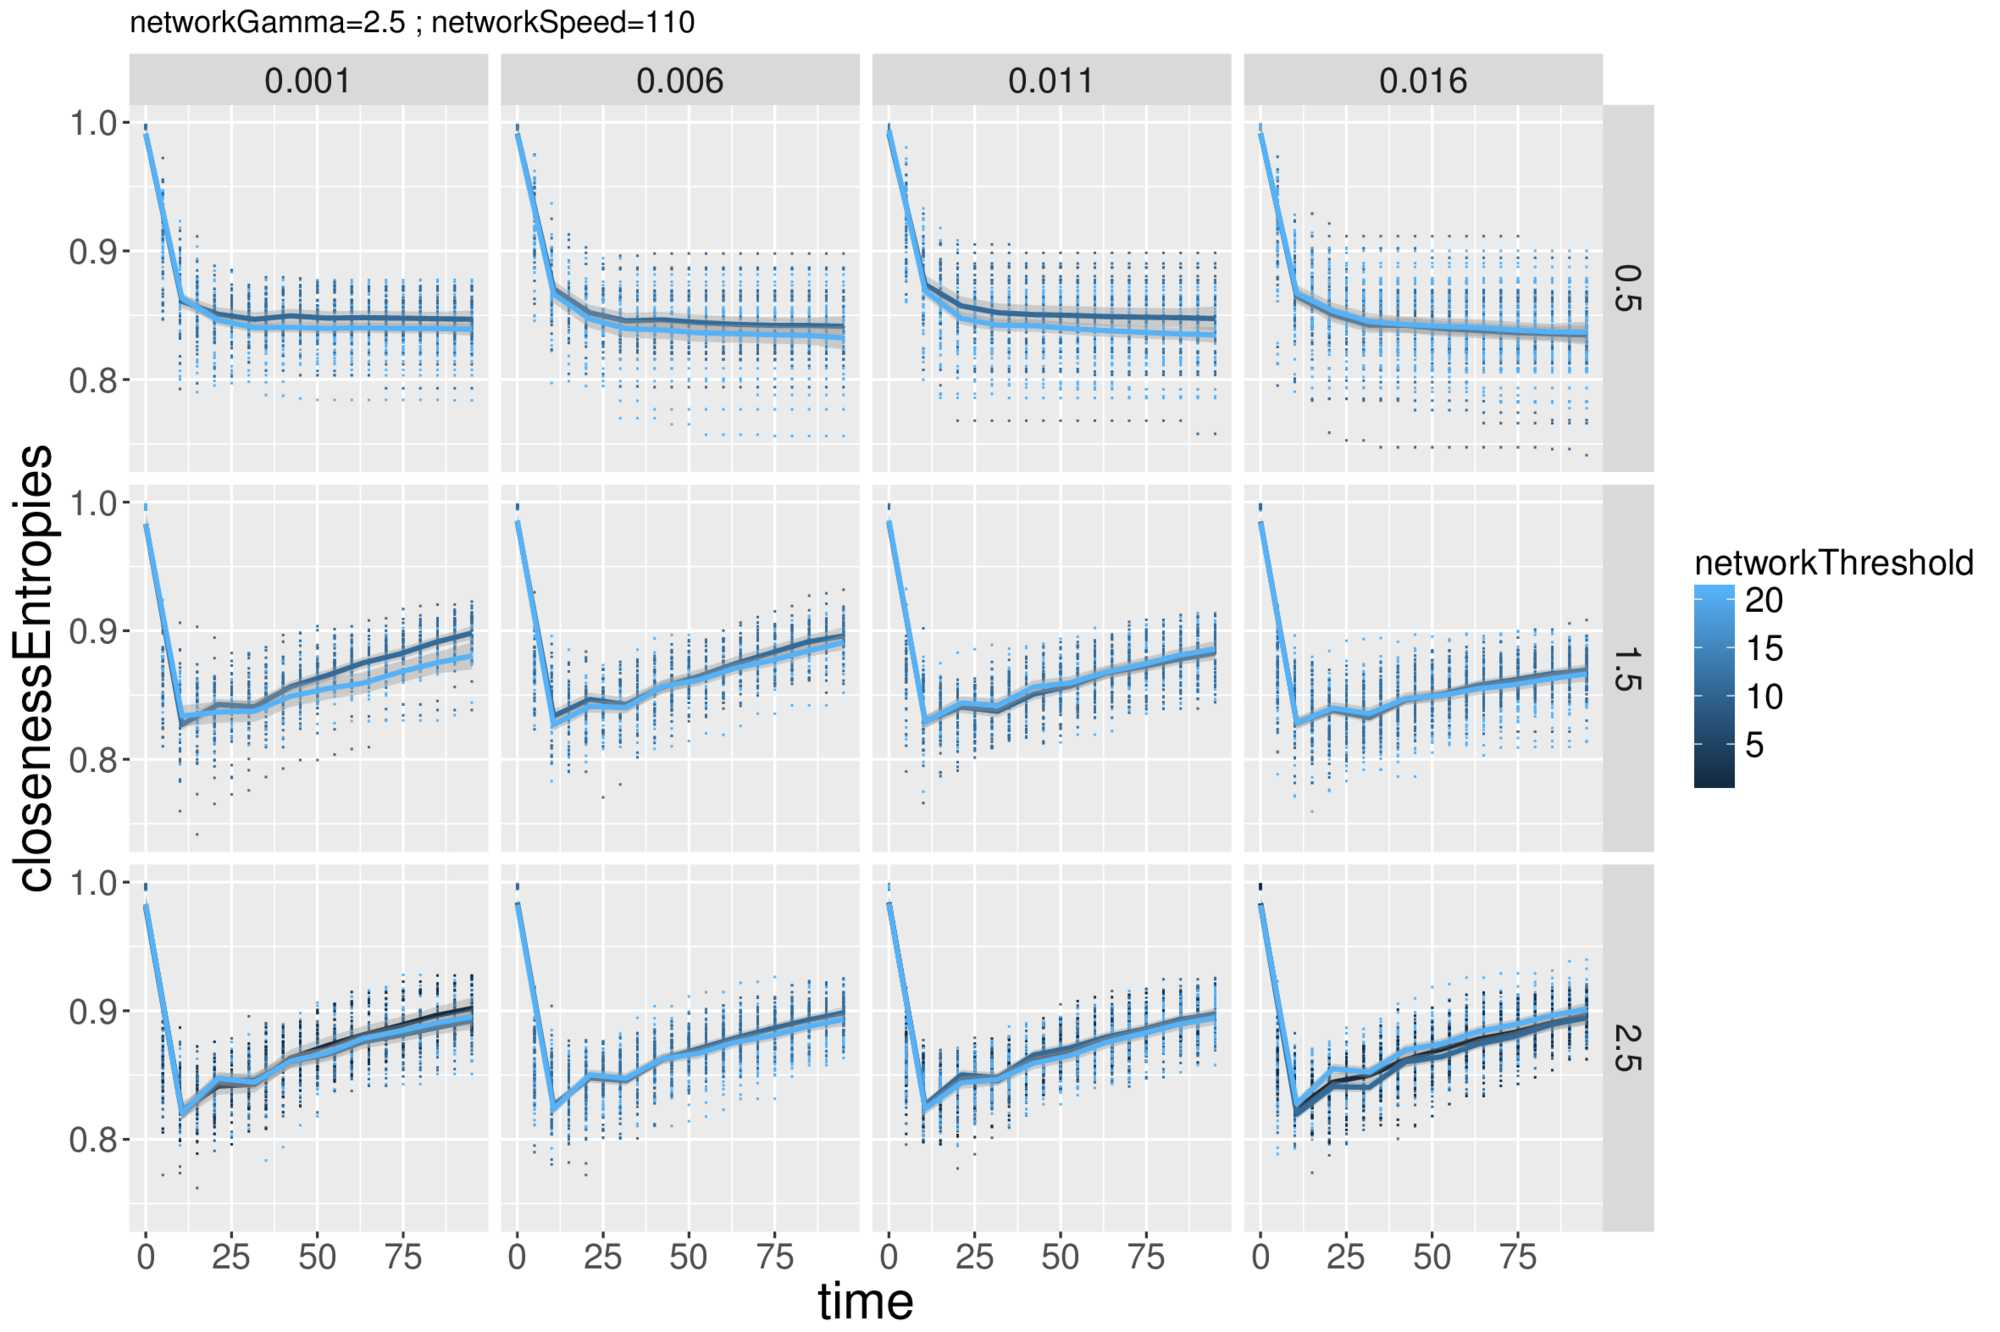
\includegraphics[width=\linewidth]{figures/A-macrocoevolexplo-closeness.jpg}
%\caption{\textbf{Entropy of closeness centralities.} We give $\varepsilon \left[\mu_i\right]$ as a function of time $t$, for $\theta_N$ variable (color), $d_G$ variable (columns) and $\gamma_G$ variable.\label{fig:app:macrocoevolexplo:closeness}}
%\end{figure}
%%%%%%%%%%%%%%%%%%

%%%%%%%%%%%%%%%%%%
%\begin{figure}
%    %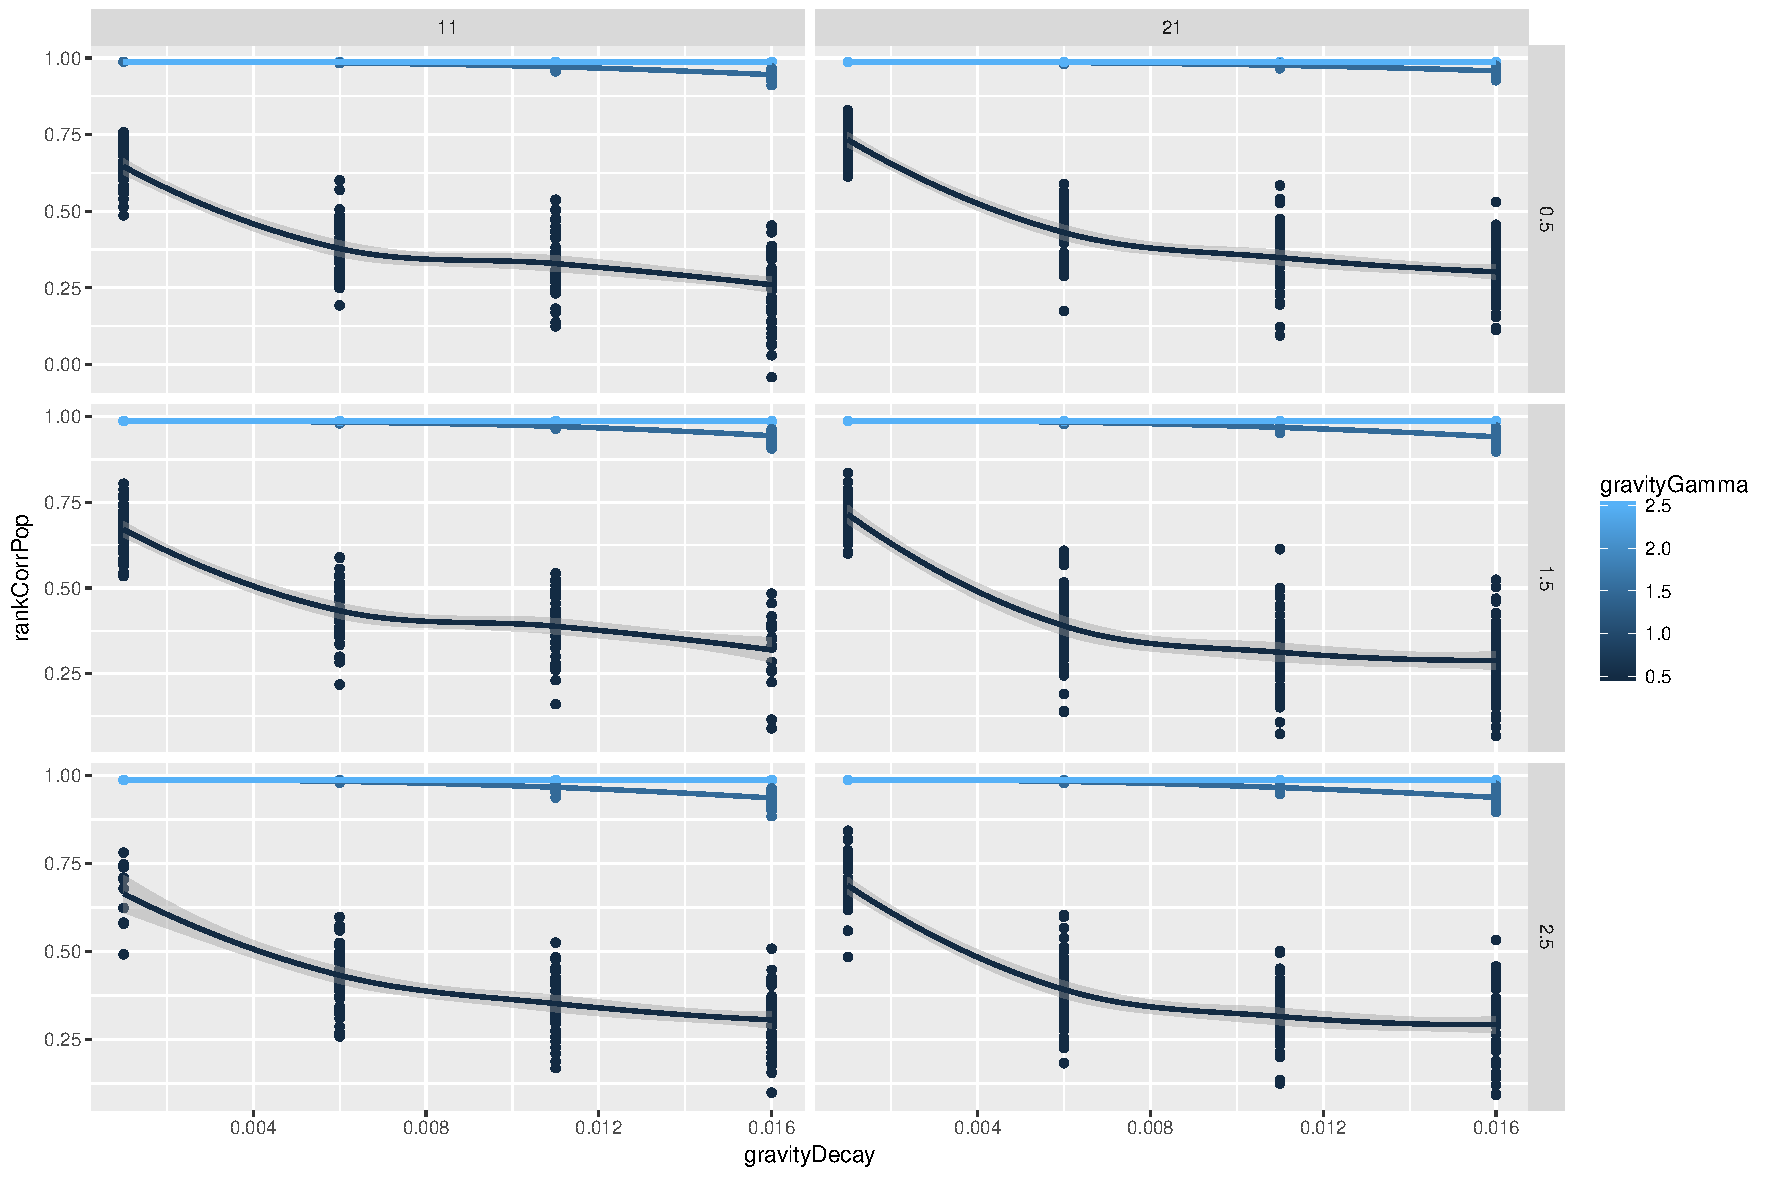
\includegraphics[width=0.48\linewidth]{Figures/MacroCoEvolExplo/rankCorrPop_synthRankSize0_5_networkSpeed10}
%    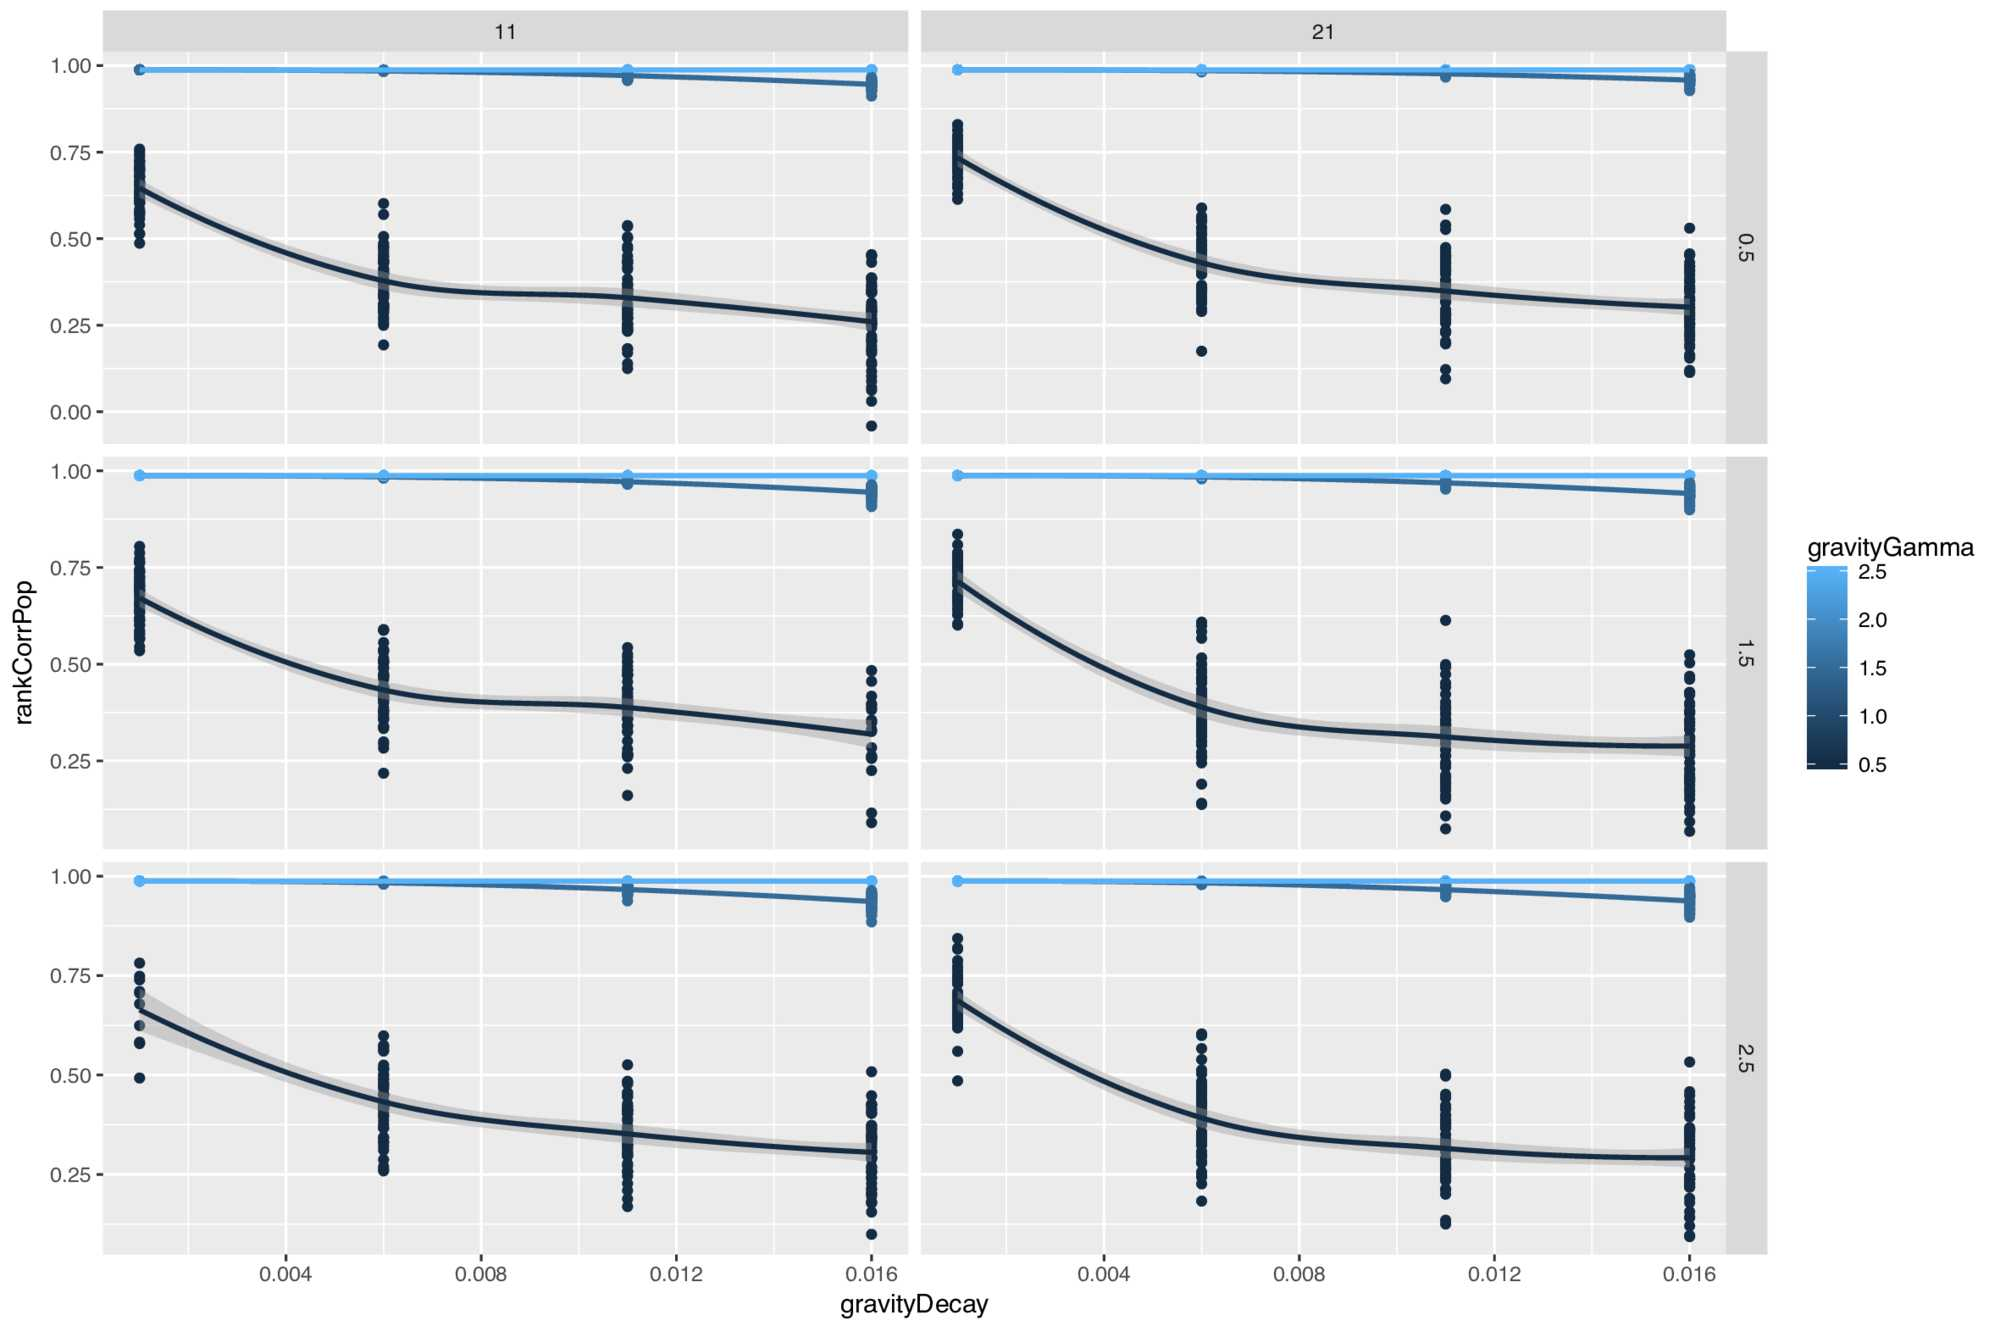
\includegraphics[width=\linewidth]{figures/A-macrocoevolexplo-rankcorrpop.jpg}
%\caption{\textbf{Population rank correlations.} We give $\rho_r \left[\mu_i\right]$ as a function of $d_G$, for $\gamma_G$ variable (color), $\theta_N$ variable (columns) and $\gamma_N$ variable (rows).\label{fig:app:macrocoevolexplo:rankcorrpop}}{\textbf{Corrélations de rang pour la population.} Nous donnons $\rho_r \left[\mu_i\right]$ en fonction de $d_G$, pour $\gamma_G$ variable (couleur), $\theta_N$ variable (colonnes) et $\gamma_N$ variable (lignes).\label{fig:app:macrocoevolexplo:rankcorrpop}}
%\end{figure}
%%%%%%%%%%%%%%%%%%
%
%%%%%%%%%%%%%%%%%%
%\begin{figure}
%	%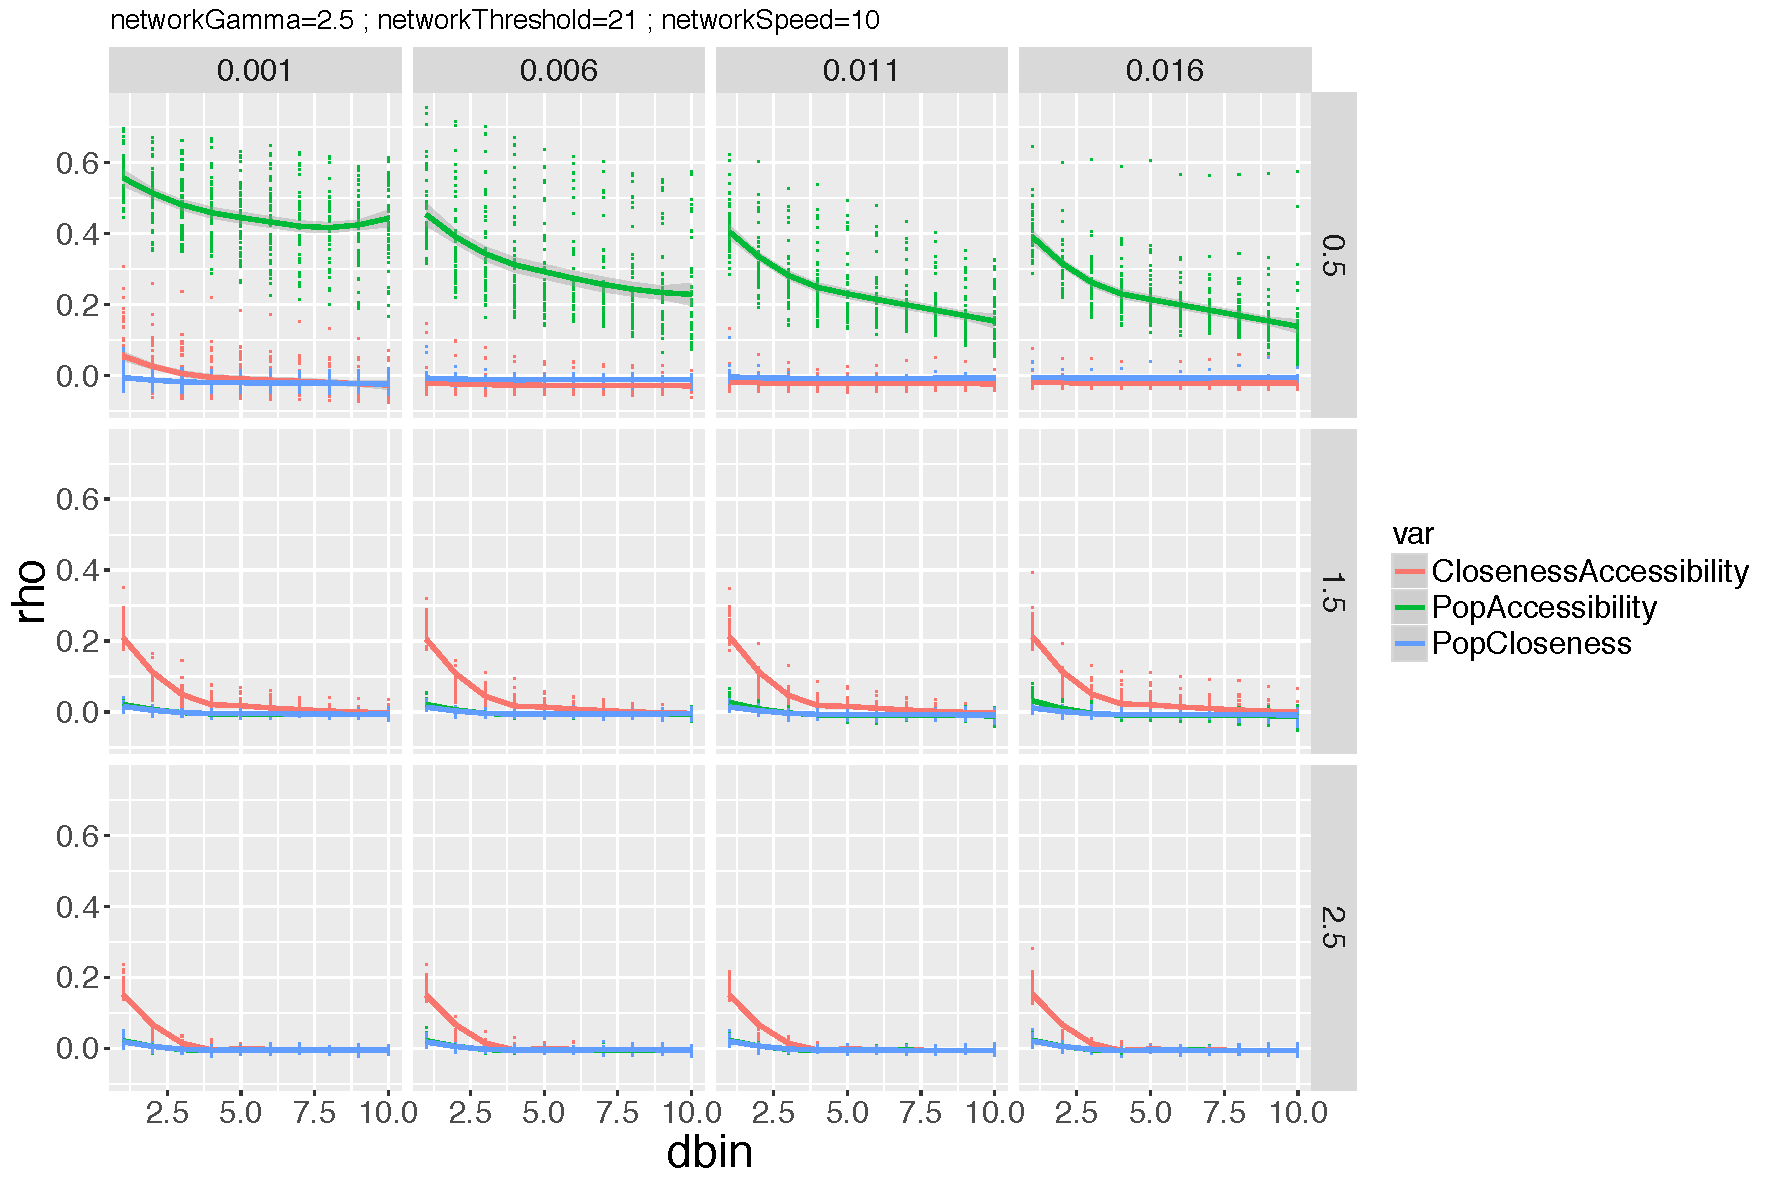
\includegraphics[width=0.48\linewidth]{Figures/MacroCoEvolExplo/distcorrs_networkGamma2_5_networkThreshold21_networkSpeed10}
%	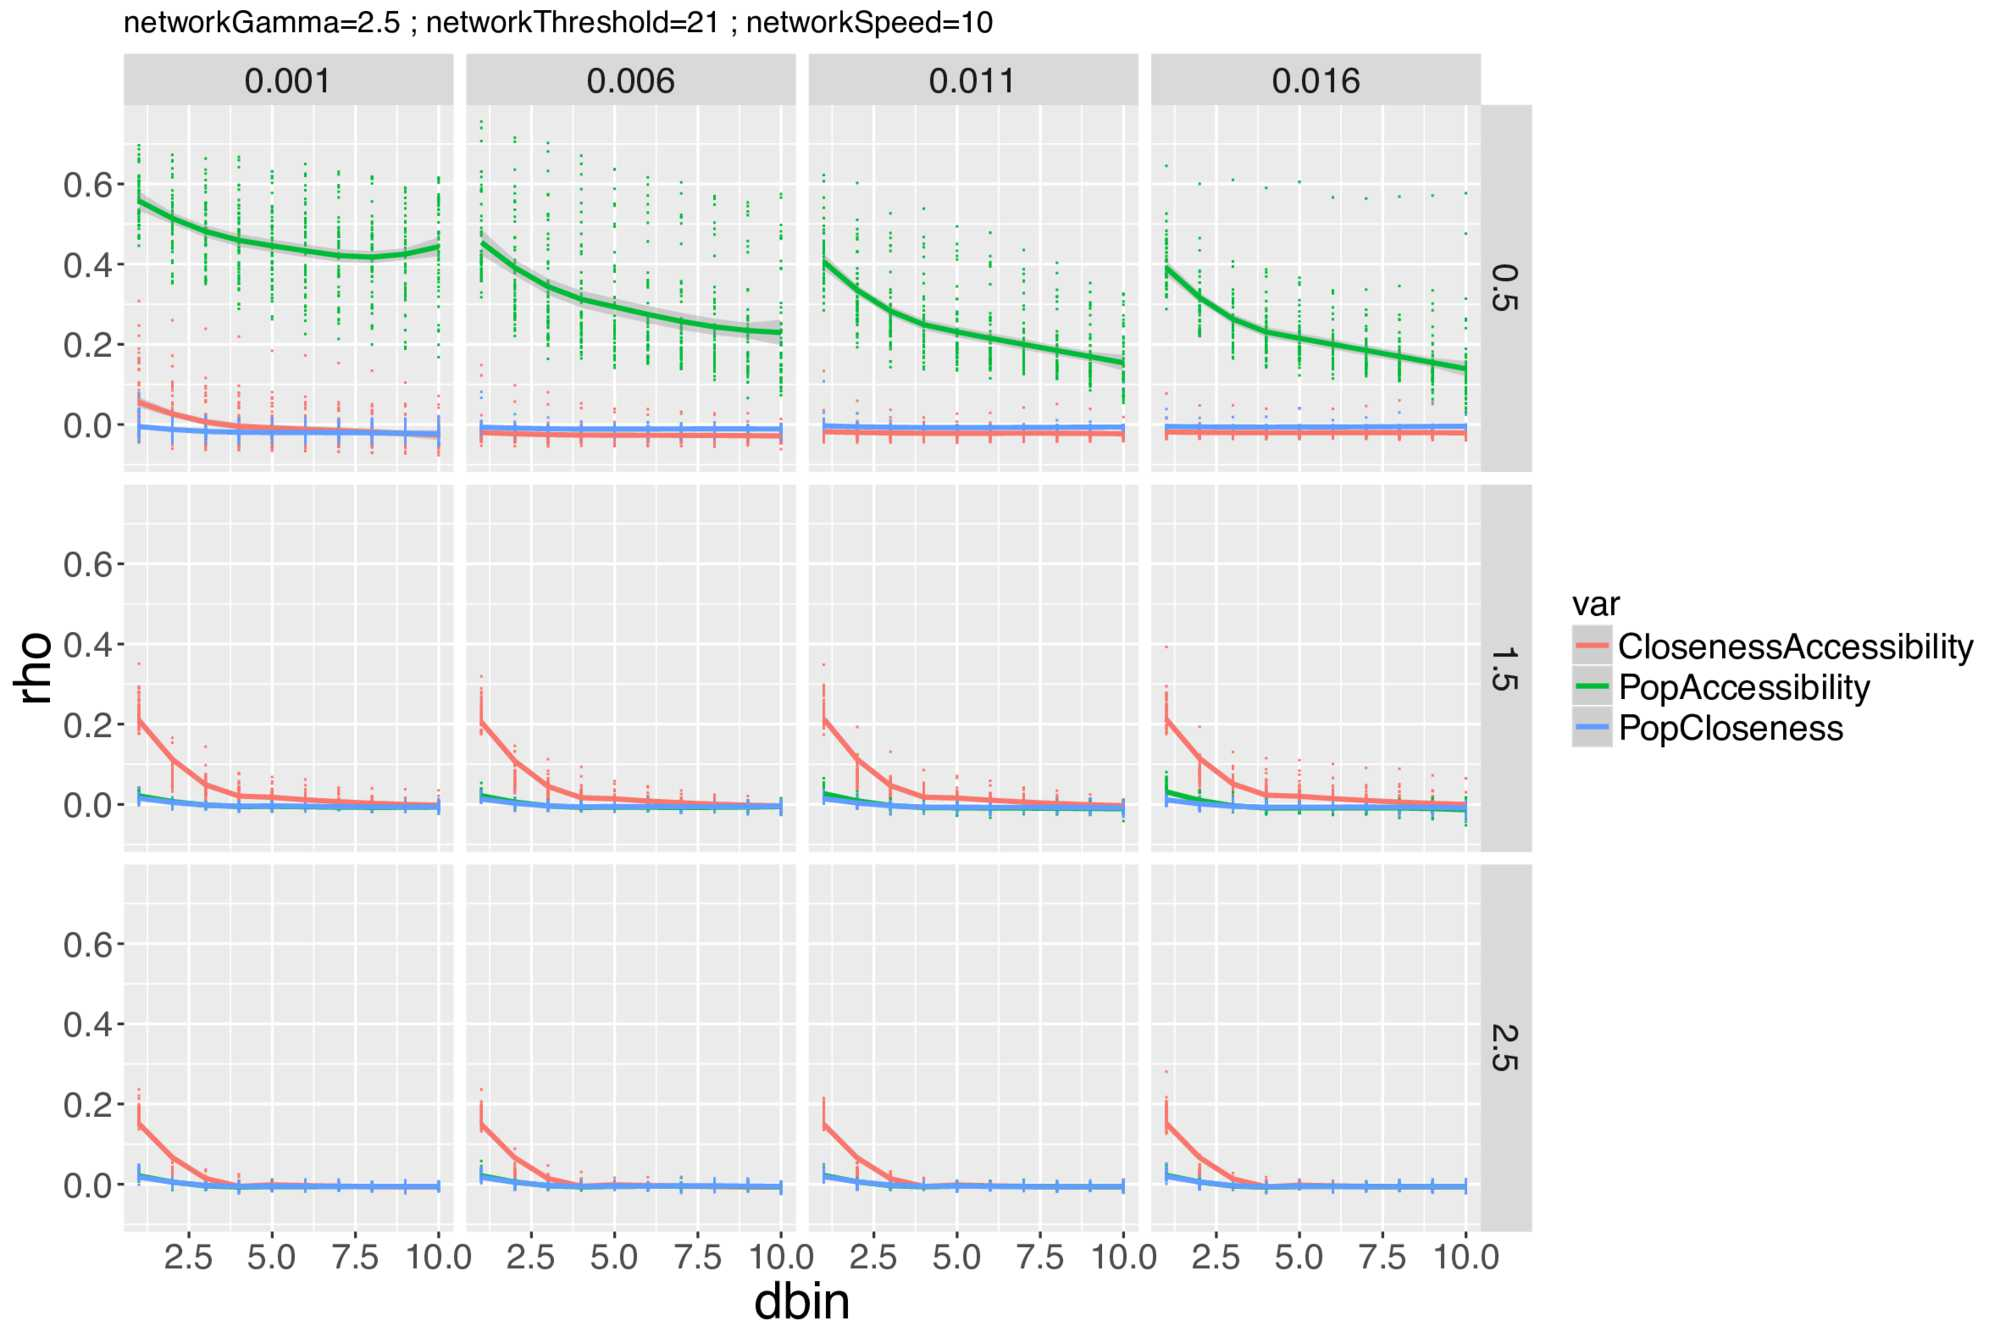
\includegraphics[width=\linewidth]{figures/A-macrocoevolexplo-distcorrs.jpg}
%	\caption{\textbf{Correlations as a function of distance.} We give correlations $\rho_d$ as a function of distance decile, for all couples of variables (color), for $d_G$ variable (columns) and $\gamma_G$ variable (rows), at fixed $\gamma_N = 2.5$, $\theta_N=21$ and $v_0 = 10$.\label{fig:app:macrocoevolexplo:distcorrs}}
%\end{figure}
%%%%%%%%%%%%%%%%%%



%
%%%%%%%%%%%%%%%%%%
%\begin{figure}
%	%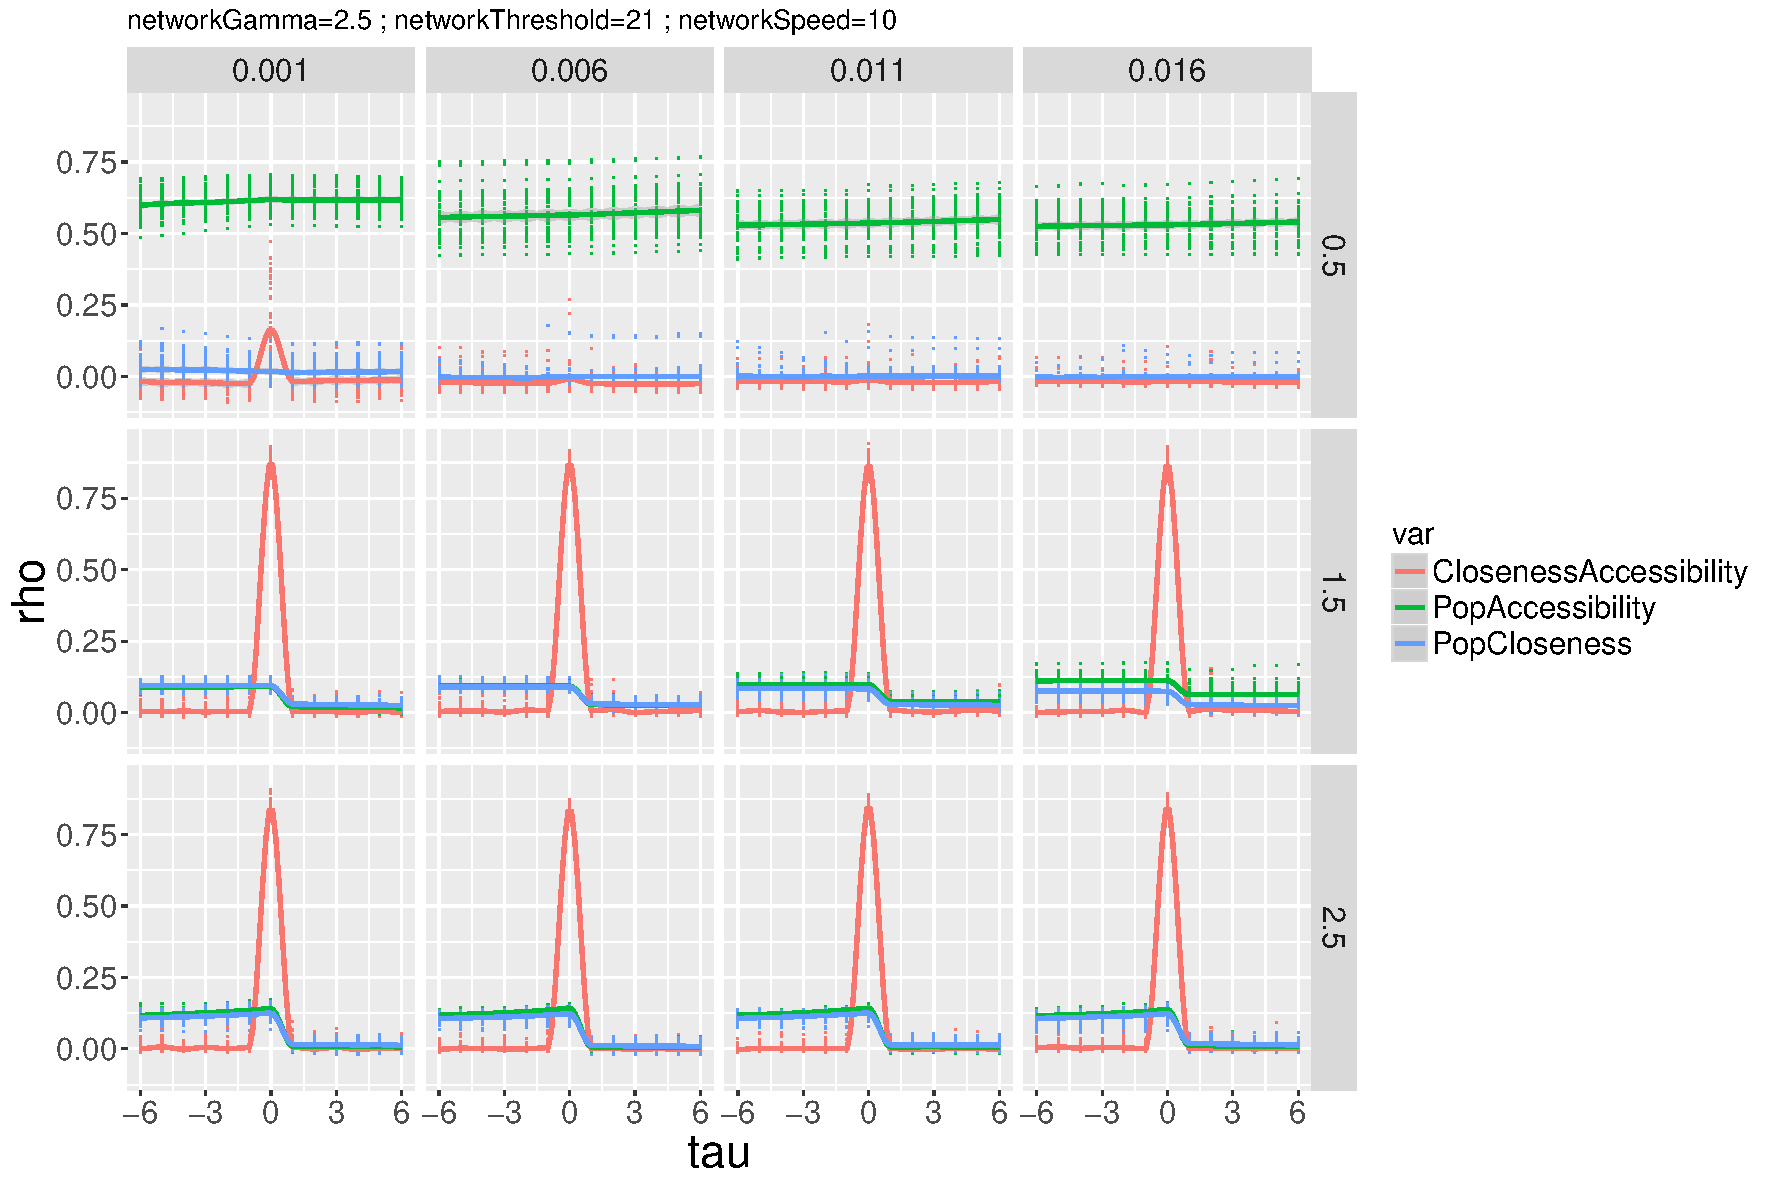
\includegraphics[width=0.48\linewidth]{Figures/MacroCoEvolExplo/laggedcorrs_networkGamma2_5_networkThreshold21_networkSpeed10}
%	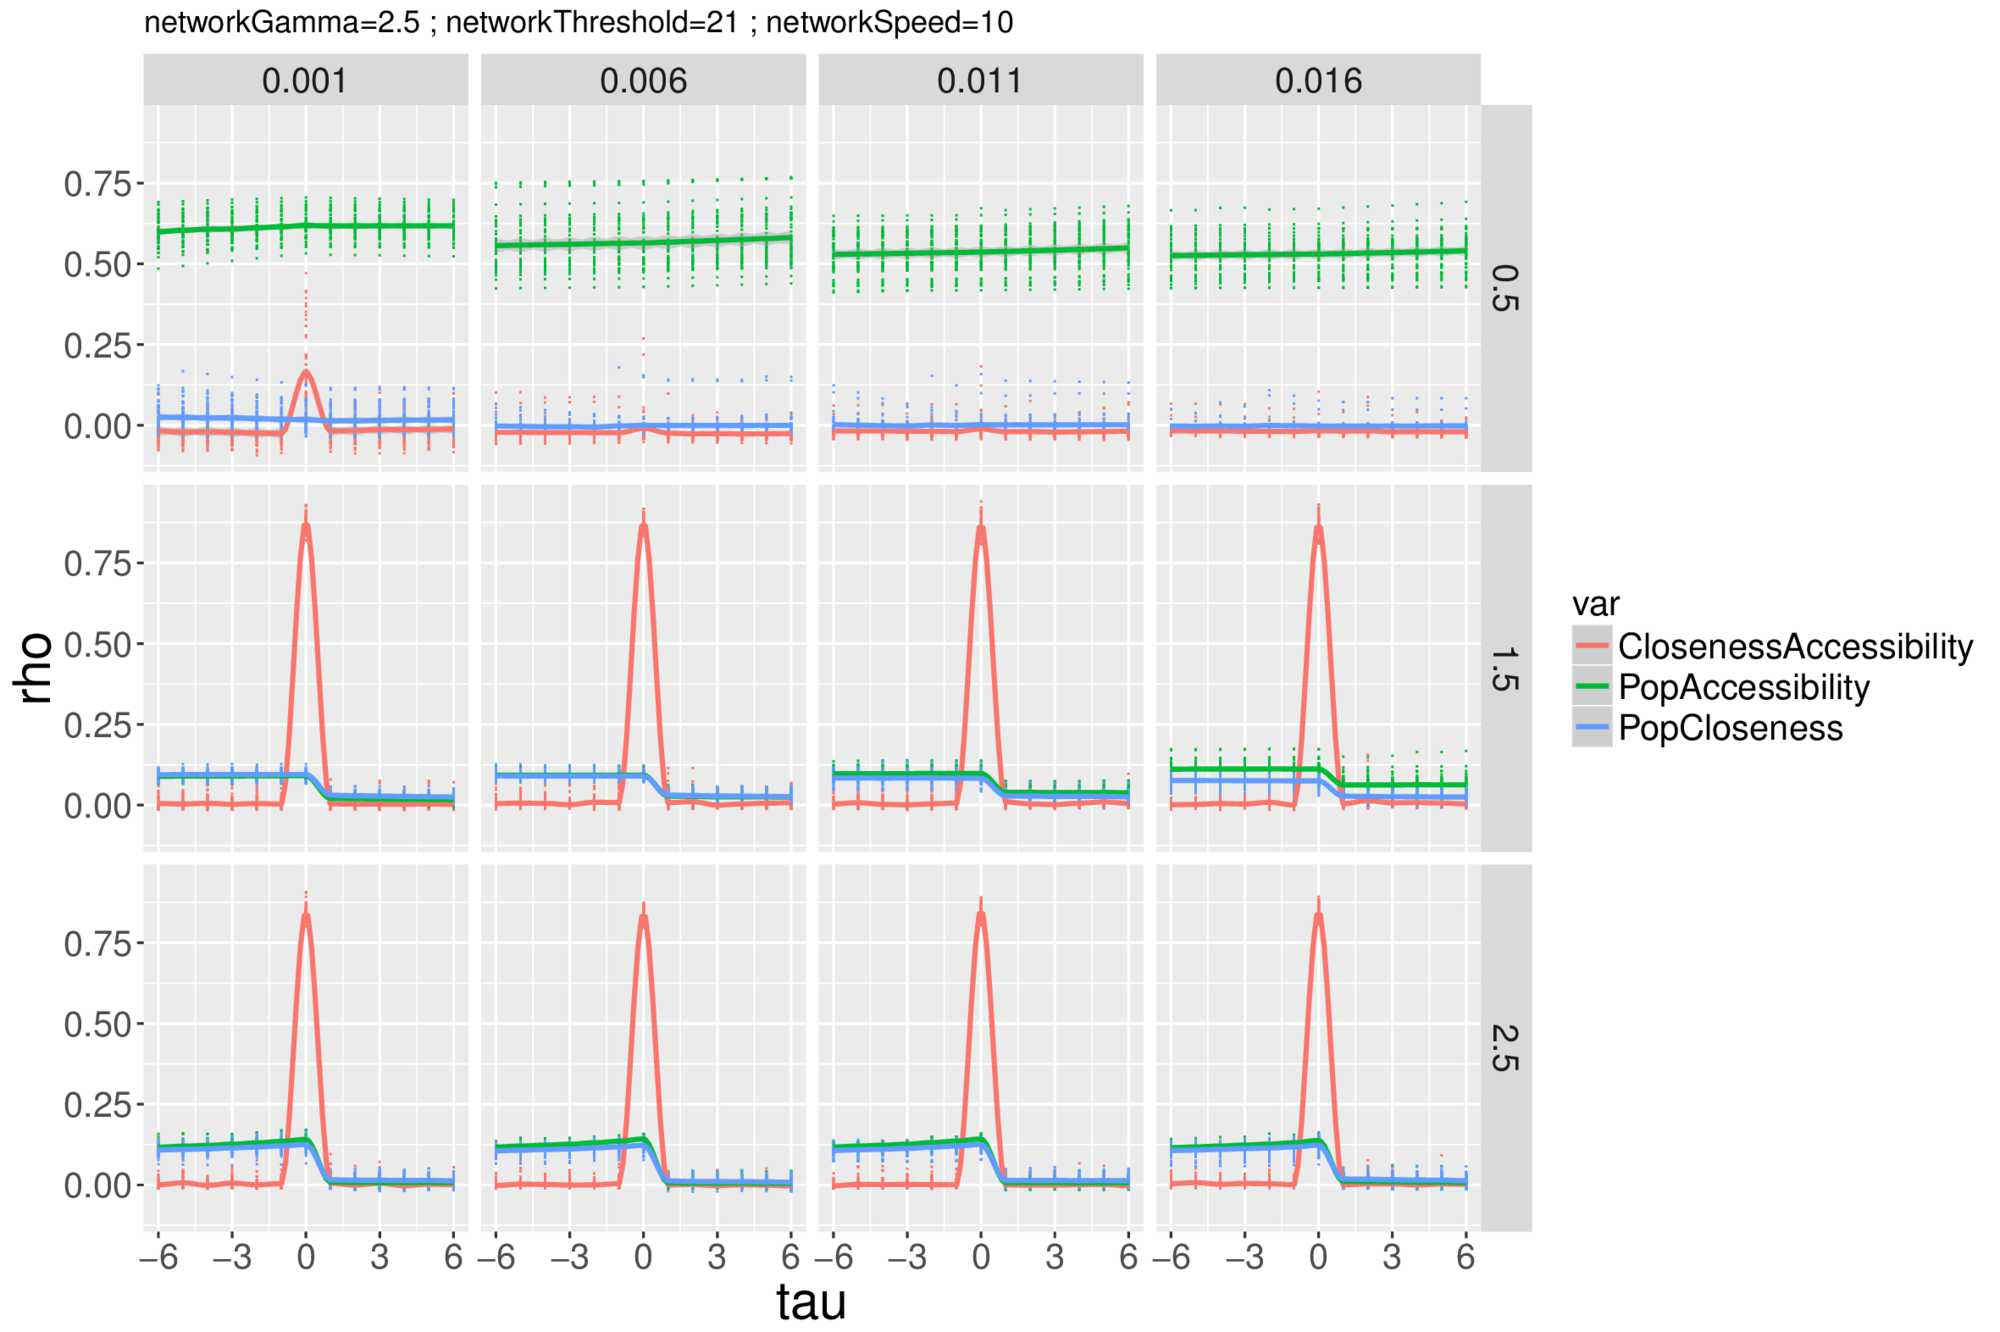
\includegraphics[width=\linewidth]{figures/A-macrocoevolexplo-laggedcorrs.jpg}
%	\caption{\textbf{Lagged correlations.} We give the lagged correlations $\rho_{\tau}$ as a function of the delay $\tau$, for all couples of variables (color), for $d_G$ variable (columns) and $\gamma_G$ variable (rows), at fixed $\gamma_N = 2.5$, $\theta_N=21$ and $v_0 = 10$.\label{fig:app:macrocoevolexplo:laggedcorrs}}
%\end{figure}
%%%%%%%%%%%%%%%%%%



%%%%%%%%%%%%%%%%%%%%
%% Biblio
%%%%%%%%%%%%%%%%%%%%

\bibliographystyle{apalike}
\bibliography{biblio}



\end{document}




%%%%%%%%%%%%%%%%%%%%%%%
%% -- TEMPLATE --
%%%%%%%%%%%%%%%%%%%%%%%
%


%
%\begin{description}[Type 1]
%\item[Type 1]{That addresses central themes pertainng to migration, health, and disease. In Sect.~\ref{sec:1}, Wilson discusses the role of human migration in infectious disease distributions and patterns.}
%\item[Type 2]{That addresses central themes pertainng to migration, health, and disease. In Sect.~\ref{subsec:2}, Wilson discusses the role of human migration in infectious disease distributions and patterns.}
%\end{description}


%
%
%% For figures use
%%
%\begin{figure}[b]
%\sidecaption
%% Use the relevant command for your figure-insertion program
%% to insert the figure file.
%% For example, with the graphicx style use
%\includegraphics[scale=.65]{figure}
%%
%% If no graphics program available, insert a blank space i.e. use
%%\picplace{5cm}{2cm} % Give the correct figure height and width in cm
%%
%\caption{If the width of the figure is less than 7.8 cm use the \texttt{sidecapion} command to flush the caption on the left side of the page. If the figure is positioned at the top of the page, align the sidecaption with the top of the figure -- to achieve this you simply need to use the optional argument \texttt{[t]} with the \texttt{sidecaption} command}
%\label{fig:1}       % Give a unique label
%\end{figure}
%



%
%% For tables use
%%
%\begin{table}
%\caption{Please write your table caption here}
%\label{tab:1}       % Give a unique label
%%
%% Follow this input for your own table layout
%%
%\begin{tabular}{p{2cm}p{2.4cm}p{2cm}p{4.9cm}}
%\hline\noalign{\smallskip}
%Classes & Subclass & Length & Action Mechanism  \\
%\noalign{\smallskip}\svhline\noalign{\smallskip}
%Translation & mRNA$^a$  & 22 (19--25) & Translation repression, mRNA cleavage\\
%Translation & mRNA cleavage & 21 & mRNA cleavage\\
%Translation & mRNA  & 21--22 & mRNA cleavage\\
%Translation & mRNA  & 24--26 & Histone and DNA Modification\\
%\noalign{\smallskip}\hline\noalign{\smallskip}
%\end{tabular}
%$^a$ Table foot note (with superscript)
%\end{table}
%%


%
%
%\begin{figure}[t]
%\sidecaption[t]
%% Use the relevant command for your figure-insertion program
%% to insert the figure file.
%% For example, with the option graphics use
%\includegraphics[scale=.65]{figure}
%%
%% If no graphics program available, insert a blank space i.e. use
%%\picplace{5cm}{2cm} % Give the correct figure height and width in cm
%%
%%\caption{Please write your figure caption here}
%\caption{If the width of the figure is less than 7.8 cm use the \texttt{sidecapion} command to flush the caption on the left side of the page. If the figure is positioned at the top of the page, align the sidecaption with the top of the figure -- to achieve this you simply need to use the optional argument \texttt{[t]} with the \texttt{sidecaption} command}
%\label{fig:2}       % Give a unique label
%\end{figure}



%Use the standard \verb|equation| environment to typeset your equations, e.g.
%
%\begin{equation}
%a \times b = c\;,
%\end{equation}
%
%however, for multiline equations we recommend to use the \verb|eqnarray| environment\footnote{In physics texts please activate the class option %\texttt{vecphys} to depict your vectors in \textbf{\itshape boldface-italic} %type - as is customary for a wide range of physical subjects}.
%\begin{eqnarray}
%a \times b = c \nonumber\\
%\vec{a} \cdot \vec{b}=\vec{c}
%\label{eq:01}
%\end{eqnarray}

%\begin{svgraybox}
%If you want to emphasize complete paragraphs of texts we recommend to use the newly defined Springer class option \verb|graybox| and the newly defined environment \verb|svgraybox|. This will produce a 15 percent screened box 'behind' your text.

%If you want to emphasize complete paragraphs of texts we recommend to use the newly defined Springer class option and environment \verb|svgraybox|. This will produce a 15 percent screened box 'behind' your text.
%\end{svgraybox}













